\chapter{Adaptive transition kernels for Bayesian phylogenetics}
\epigraph{ 
Monte Carlo is an extremely bad method; it should be used only when all alternative methods are worse.
}{Alan Sokal (1955-) in \textit{Monte Carlo Methods in Statistical Mechanics: Foundations and New Algorithms} (1996).}


\section{Introduction}	
\label{sec:intro_ch2}

In Bayesian phylogenetics one is usually interested in computing the posterior distribution
\begin{equation}
\label{eq:posterior}
 p(t, \boldsymbol b, \boldsymbol \theta | D) = \frac{f(D | t, \boldsymbol b, \boldsymbol \theta ) \pi(t, \boldsymbol b, \boldsymbol \theta )}{\sum_{t_i \in \mathbb{F}} \int_{\boldsymbol B}\int_{\boldsymbol \Theta} f(D | t_i, \boldsymbol b_i, \boldsymbol \theta ) \pi(t_i, \boldsymbol b_i, \boldsymbol \theta ) d\boldsymbol\theta d\boldsymbol b_i}\:,
\end{equation}
where $D$ is observed data and $t \in \mathbb{F}$ is a fully-ranked tree topology associated set of branch lengths $\boldsymbol b$. %TODO: maybe $\boldsymbol b(t)$?
Finally $\boldsymbol \theta$ is a set of parameters such as substitution model parameters, migration rates, heritability coefficients, etc.
In many applications, the aim is to construct time-calibrated phylogenies, i.e. phylogenetic trees whose branch lengths are measured in units of calendar time.
In particular, one might have sequences sampled through time (heterochronous) which enable direct estimation of the rate of evolution and reconstruction of past population dynamics~\citep{Drummond2002, Drummond2005}.
These types of data sets pose additional challenges to inference because they impose constraints\footnote{More specifically temporal precedence constraints.} on the space of valid trees~\citep{Stadler2013}.

\subsection{MCMC in phylogenetic space}
\label{sec:tree_mcmc}

One of the main features of the Bayesian  approach is to allow parameter inference and hypothesis testing whilst accommodating phylogenetic uncertainty~\citep{Suchard2001, Huelsenbeck2002, Lemey2014, Cybis2015, Baele2015, Baele2017}.
This treatment of uncertainty is achieved by integrating (marginalising) over the space of phylogenies, which depends crucially on efficiently traversing tree space.
Even for the simplest models, the distribution in~(\ref{eq:posterior}) cannot be computed analytically -- except for exhaustive iteration of all possible tree topologies --, requiring numerical approximation, usually accomplished through Markov chain Monte Carlo (MCMC).
The use of MCMC for Bayesian methods in phylogenetics has grown steadily since its introduction in the late 1990s and early 2000s~\citep{Kuhner1995,Sinsheimer1996, Rannala1996, Yang1997, Mau1999, Li2000, Suchard2001,Drummond2002}, with software packages such as Mr Bayes~\citep{Ronquist2012} and BEAST~\citep{Drummond2012} becoming widely used by researchers in a broad range of disciplines~\citep{Murphy2001, Bouckaert2012, Lemey2014}.

The Metropolis-Hastings (MH) algorithm~\citep{Metropolis1953, Hastings1970} is a very popular MCMC technique due to its generality and ease of implementation.
% In MH, a Markov chain is constructed such that its limiting distribution is the desired posterior distribution. 
For ease of presentation, let $\tau = \{ t, \boldsymbol b\}$ be a phylogeny and $q_{\gamma}(\tau^\prime|\tau)$ be a conditional distribution indexed by a parameter $\gamma$ from which a new state $\tau^\prime$ can be proposed from a current state $\tau$, which we call a \textbf{candidate-generating distribution}.
It can be shown that accepting/rejecting a new state $\tau^\prime$ based on the ratio\footnote{I will drop the dependence of the posterior on $\boldsymbol\theta$ for convenience of notation. One should however keep in mind some parameters are strongly correlated with the phylogeny $\tau$.} $A_{\gamma}(\tau | \tau^\prime) = min\left(1, \frac{p(\tau^\prime | D)q_{\gamma}(\tau|\tau^\prime)}{p(\tau | D)q_{\gamma}(\tau^\prime|\tau)}\right)$ leads to the desired distribution for a suitably constructed proposal mechanism.

There are no ``default'' choices for the candidate-generating distribution $q_{\gamma}(\cdot|\cdot)$; it must be chosen with the target distribution (in this case the Bayesian posterior) in mind.
Moreover, the efficiency of MCMC algorithms in approximating the target distribution depends crucially on the choice of transition kernel~\citep{Brooks2003,AlAwadhi2004,Yang2013,Thawornwattana2017}.
As argued by~\cite{Hoehna2012}, tree transition kernels are usually built in a relatively simplistic fashion, which in turn leads to inefficient exploration of tree space.
Moreover, most transition kernels proposed to date are not adaptive, i.e., the parameter(s) $\gamma$ cannot be adjusted during the Markov chain to achieve a desired acceptance probability~\citep{Haario2001}.
Given the clear advantage of adaptive MCMC over non-adaptive implementations for high-dimensional target distributions~\citep{Roberts2009, Baele2017}, the development of adaptive tree transition kernels could lead to substantial gains in performance.

\cite{Hoehna2008} developed new ``clock-constrained'' transition kernels to improve efficiency when dealing with time-calibrated trees. 
The authors point out that clock-constrained trees impose additional restrictions on the state space of the MCMC algorithm and hence that performance could be increased by developing transition kernels that took the extra information provided by tip dates.
They develop two such kernels: Fixed node-height Prune-and-Regraft (FNPR) and Intermediate Exchange (IE).
FNPR finds a ``target'' node (excluding the root and its two children) at random, prunes it and regrafts the resulting subtree at a ``destination'' node in the tree at the same height at random.
Intermediate Exchange is similar in spirit, but the regraft node  is not chosen at random. 
Instead, IE is constructed to prefer local rearrangements, by picking closer nodes with a higher probability (see below and section II in~\cite{Hoehna2008} for details).
A limitation of FNPR nor IE is that they are not adaptive.

\cite{Hoehna2012} explored more sophisticated ``guided'' tree transition kernels, inspired by Gibbs sampling~\citep{Geman1984}.
The idea behind their ``Metropolised'' Gibbs samplers is to maximise transition probability, i.e., the probability that the chain moves to a new state.
This is accomplished by prohibiting the current state as a proposed state, leading to a transition probability of one.
The kernels developed in~\cite{Hoehna2012} use a weighting scheme based on conditional clade probabilities (CCP) to guide transitions between trees.
A move to a tree with a lower CCP score is thus less likely, whilst a move that increases the score has a higher probability of being accepted.
A limitation of these metropolised transition kernels is that CCP scores require normalisation over all trees~\citep{Larget2013} and hence can be cumbersome to calculate.

More recently,~\cite{Dinh2016} and~\cite{Fourment2017} develop ``guided'' candidate-generating mechanisms for on-line Bayesian phylogenetics via sequential Monte Carlo, which makes use of a surrogate function to make computations feasible.
While that is an active field of research, it relies on machinery not yet extended to the time-calibrated case.
Hence in this thesis and chapter I will focus on extending existing MH algorithms, which I will argue strikes a balance between computational efficiency and tractability.

To achieve maximum efficiency, a tree transition kernel needs to have the following characteristics: (i) be computationally cheap; (ii) be adaptive; (iii) traverse phylogenetic space quickly, i.e., have a high \textit{mixing rate}.
In this chapter I develop and study two simple, adaptive time-tree transition kernels, which we implement in the open source software package BEAST (\url{https://github.com/beast-dev/beast-mcmc/}).
I analyse performance in real as well as simulated data sets, focusing on the inference of time-calibrated phylogenies.
Technical details necessary to make some of the claims in this chapter precise are given in Section~\ref{sec:stx_properties}. %TODO: check if necessary

% \section{Technical details}
% \label{sec:tech}

\section{New time-tree transition kernels}
\label{sec:newKernels}

In this section I introduce two new candidate-generating densities that attain the properties discussed above while being specially designed for time-calibrated phylogenies.

\subsection{Preliminaries}
\label{sec:prelim}

I briefly lay out some notation and background that will be necessary for the presentation, with further details and more rigorous definitions already given in Chapter 1 (Section~\ref{sec:tree_space}).
Throughout this  chapter I will use $\boldsymbol\Psi$ to denote the parameter space encompassing topologies and branch lengths, henceforth called ``phylogenetic space'', and $\tau \in \boldsymbol\Psi$ to denote a bifurcating, rooted tree with branch lengths on $n$ taxa\footnote{What~\cite{Drummond2015} call a ``fully ranked'' tree.}.
Let $\mathbf{B}(\tau) =\{b_1, b_2, \ldots, b_{2n-2}\}$ be the set of branch lengths of $\tau$.
It is possible to compute the height of each node using a mapping $h(\cdot)$ such that $\mathbf{H}(\tau) = \{h_1, h_2, \ldots, h_{2n-1}\}$ is the set of node heights for all nodes (internal and external) in $\tau$.
Here we will define $h(i) = l_{max} - l_i$ and $l_i = \sum_{k \in \mathbf{W_i}} b_k$, where $\mathbf{W_i}$ is the minimal path between node $i$ and the root $\rho$ and $l_{max}$ is the maximum of these shortest paths.
It is also convenient to define $P_i$, $G_i$ and $S_i$ as the parent, grandparent and sibling of node $i$, respectively.
With this notation in mind, call $p_i = h(P_i)-h(i)$, $g_i = h(G_i)-h(P_i)$ and $q_i = h(P_i)-h(S_i)$ the corresponding branch lengths.
The most recent common ancestor of nodes $i$ and $j$, $\text{mrca}_{ij}$ is the first node in which the paths $\mathbf{W_i}$ and $\mathbf{W_j}$ intersect.
Finally, let $d(i, j) = 2h(\text{mrca}_{ij}) - [ h(i)  + h(j) ]$ be the patristic (path) distance between nodes $i$ and $j$ on the phylogeny.

\subsubsection*{SubTreeJump} 

The first transition kernel I propose, \textit{SubTreeJump} (STJ)\footnote{An alternative name for STJ is generalised fixed node height prune and regraft, gFNPR.}, is similar in spirit to both Intermediate Exchange and FNPR.
STJ extends IE by introducing a tuning parameter $\alpha$ that controls how local rearrangements are.
The idea is to make the probability of moving node $i$ to $j$ proportional to $l_{ij}^\alpha$ instead $l_{ij}$ as in Intermediate Exchange.
The necessary steps to perform a SubTreeJump operation on $\tau$ in order to propose a phylogeny $\tau^\prime$ are described in detail in Box~\ref{alg:stj} and an illustration is provided in Figure~\ref{fig:stj}.
This allows one to favour bold moves away from $i$ ($\alpha > 0$) or more conservative moves closer to $i$ ($\alpha < 0$).
Notice that SubTreeJump is equivalent to FNPR for $\alpha = 0$.
One can then define the SubTreeJump candidate-generating density as $q_{\alpha}(\tau^\prime | \tau) = Pr(i\to j)$.

\begin{algorithm}[!ht]

\setcounter{AlgoLine}{-1}

 Excluding the root and its children, pick a node $i$ in  $\tau$ uniformly at random, i.e., with probability $1/(2n-4)$;
 
 Determine $P_i$ and compute $h(P_i)$;
 
 Construct the set of destination nodes $\mathbf{D_i} = \{ d \in \mathbf{D_i}  : h(d) \leq h(P_i) < h(P_d) \}$;
 
 For all $k \in \mathbf{D_i}$, compute $l_{ik}$;
 
 For some fixed $\alpha \in \mathbb{R}$, pick a node $j$ with probability $Pr(i\to j) = \frac{(l_{ij})^{\alpha}}{\sum_{d \in \mathbf{D_i}}(l_{id})^{\alpha}}$;
 
 Prune the phylogeny at $P_i$ and regraft the resulting subtree at $P_j$, creating a new phylogeny $\tau^\prime$. 
 
 \caption{SubTreeJump transition kernel.}
 \label{alg:stj}
\end{algorithm}

Note that while for $\alpha = 0$ the move is symmetric~\citep{Hoehna2008}, for $\alpha \neq 0$ the density $q_{\alpha}(\cdot|\cdot)$ is not, since for two arbitrary nodes $i$ and $j$  whilst the sets $\mathbf{D_i}$ and $\mathbf{D_j}$ coincide ($|\mathbf{D_i}| = |\mathbf{D_j}|$), the distances between nodes usually do not.
Hence one needs to compute the \textit{Hastings ratio} $q_{\alpha}(\tau|\tau^\prime)/q_{\alpha}(\tau^\prime|\tau)$.
To get a reverse move from $\tau^\prime$ back to $\tau$, one needs to pick the original target node $i$  -- which is guaranteed to exist in $\mathbf{D_j}$ -- as a destination. 
The Hastings ratio is then\footnote{Note that I omit the node-picking probability $1/(2n-4)$ because it is the same for both moves. If one were to devise a kernel with non-uniform node-picking probabilities, these would have to be included in the Hastings ratio.}
\begin{align}
 \frac{q_{\alpha}(\tau| \tau^\prime)}{q_{\alpha}(\tau^\prime| \tau) }  &= \frac{(l_{ji})^{\alpha}}{\sum_{d^\prime \in \mathbf{D_j}}(l_{jd^\prime})^{\alpha}} /\frac{(l_{ij})^{\alpha}}{\sum_{d \in \mathbf{D_i}}(l_{id})^{\alpha}}, \nonumber \\
 &  = \frac{\sum_{d \in \mathbf{D_i}}(l_{id})^{\alpha}}{\sum_{d^\prime \in \mathbf{D_j}}(l_{jd^\prime})^{\alpha}}.
\end{align}

I note two limitations of this transition kernel.
First, because $\mathbf{H}(\tau)$ is ultimately discrete for any given $\tau$, not any acceptance probability is attainable.
This ``granularity'' of the kernel density causes problems for most adaptation schemes because the dependence of the acceptance probability on the indexing parameter is implicitly assumed to be smooth (see Section~\ref{sec:STJadap}).
% becomes irrelevant for large trees, but remains an issue for very small trees ($<10$ taxa).
Secondly, SubTreeJump on its own does not necessarily induce an irreducible Markov chain on the space of rooted topologies  -- see Section~\ref{sec:stx_properties} for a counterexample/proof.
This can be easily remedied by combining STJ with branch length candidate-generating mechanisms.
%TODO: MAS: It is not the transition kernel w.r.t.~the topology $\tau$ that concerns me much.  It's the kernel w.r.t.~the inter-coalescent intervals (the natural parameterization of our priors) that we need to confirm.
Since STJ  (and FNPR) does not change node heights or numbers of lineages, it does not change the density under the coalescent prior,~\textit{i.e.} $\pi(\tau) = \pi(\tau^\prime)$.
Whether this is a desirable property is an open question.
The disconnect between proposals in topological space and branch length space could be undesirable due to it failing to account for the dependence between topology and branch lengths.

\begin{figure}[!ht]
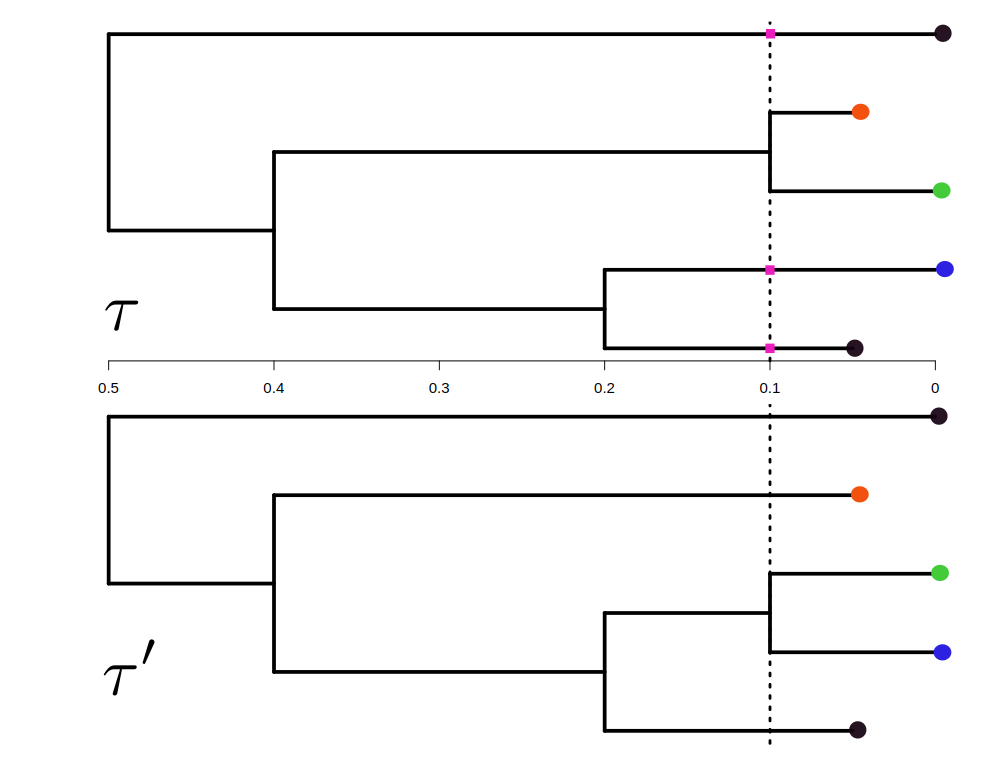
\includegraphics[scale=0.5]{\dir/figs/STJ.pdf}
 \caption[Schematic representation of a SubTreeJump proposal]{\textbf{Schematic representation of a SubTreeJump proposal}. The target node (green) is picked, we find all the nodes (or positions along branches) that intersect at the height of its parent (pink squares) and then a destination is picked with probability as described in the text.
 Other nodes are coloured so the reader can easily identify the changes.}
 \label{fig:stj}
\end{figure}


\subsubsection*{SubTreeLeap} 

Ideally, we would like to have a single adaptive transition kernel to update topology and branch lengths simultaneously.
To this end I propose~\textit{SubTreeLeap} (\verb|STL|), a transition kernel based on patristic distances.
The central idea behind \verb|STL| is to move a node $i$ to new location in the tree that is at most at (patristic) distance $\delta$ from $i$.
To this end, one first draws the distance $\delta$ from a distribution $\kappa(\delta | \sigma)$ indexed by a parameter $\sigma$, henceforth called the \textit{distance kernel}.
One then finds the set $\mathbf{D_i(\delta)}$ of all the destination nodes that are at distance $\delta$ from $i$, and picks the destination $j$ uniformly at random from these.
The regraft height of $j$ -- at $P_j$ -- will be $h^\prime = 2 h(\text{mrca}_{ij}) - h(P_i) -\delta$.
See Box~\ref{alg:stl} for details.

\begin{algorithm}[!ht]
\setcounter{AlgoLine}{-1}
\SetKwProg{Fn}{Function}{}{}
\SetKwInOut{In}{Input}
\SetKwInOut{Out}{Output}

     Excluding the root, pick a node $i$ in  $\tau$ uniformly at random, i.e., with probability $1/(2n-2)$;
     
     Draw a patristic distance $\delta$ from the distance kernel $\kappa(\delta | \sigma)$;
     
     Find the set of destination nodes $\mathbf{D_i}(\delta) \leftarrow getDestinations(\tau, i, \delta)$;
     
%      \eIf{$\mathbf{D_i}(\delta) = \O$}{
%      Prune $p_i$ and regraft it at height $h_{b} =  h(p_i) - \delta$, creating a new tree $\tau^\prime$.
%      }{
     Pick a node $j \in \mathbf{D_i}(\delta)$ with probability $Pr(i\to j) = 1/|\mathbf{D_i}(\delta)|$;
     
     Prune the tree at $P_i$ and regraft it at $P_j$, creating a new tree $\tau^\prime$. %% TODO: should it be "prune the tree at $i$" ??
%      }
     
     \Fn{getDestinations}{
     \In{ A tree $\tau$, a node $i$ and a scalar $\delta$.}
     \Out{A set $\mathbf{D_i}(\delta) = \{c \in \mathbf{D_i}(\delta)  : d(c, i) \leq \delta \}$.}
     \setcounter{AlgoLine}{-1}
     
      Determine $P_i$, $S_i$ and $G_i$;
      
      Compute $p_i = h(P_i)$;
      
      Compute $h_{b} =  p_i - \delta$; 
     
      \If{$h_b > h(i)$}{
         Go down the subtree subtended by $s_i$ and find all nodes that intersect at height $h_b$ constructing the set $\mathbf{D^{(b)}_i} = \{ d \in \mathbf{D^{(b)}_i}  : h(d) \leq h_b < h(P_d) \}$\;
    }
      Compute $h_{a} =  h(P_i) + \delta$;
      
      Walk up to the root and find all nodes that intersect at height $h_a$ constructing the set $\mathbf{D^{(a)}_i} = \{ d \in \mathbf{D^{(b)}_i}  : h(d) \leq h_b < h(P_d) \}$\;
      
    \Return $\mathbf{D_i}(\delta) = \mathbf{D^{(b)}_i}(\delta) \cup \mathbf{D^{(a)}_i(\delta)} $
     }
     
 \caption{SubTreeLeap transition kernel.}
 \label{alg:stl}
\end{algorithm}

\begin{figure}[!ht]
\begin{center}
\includegraphics[scale=0.25]{\dir/figs/STL_new.pdf} 
\end{center}
% \begin{center}
% \subfigure[\textbf{Symmetric example}]{\includegraphics[scale=0.4]{\dir/figs/STL_new.pdf} }%
% \subfigure[\textbf{Asymmetric example}]{\includegraphics[scale=0.4]{\dir/figs/STL_new.pdf} }  
% \end{center}
 \caption[Schematic representation of a SubTreeLeap proposal]{\textbf{Schematic representation of a SubTreeLeap proposal}.
 SubtreeLeap operation with size  $\delta^\prime = 1.6$ on $\tau$ to obtain the proposal phylogeny $\tau^\prime$.
 Target node represented by the green triangle and the height of its parent (green circle) marked by a dotted line; valid destination nodes marked with pink squares, invalid (prohibited) with black squares.
%  Starting from a phylogeny $\tau$, excluding the root pick a node $i$ uniformly at random (red triangle) and distance $\delta^\prime = 1.6$ from the kernel $\kappa(\delta | \sigma)$ (blue distribution).
%  Find the possible destination(s) that are distance $\delta^\prime$ from $P_i$, whose height is marked with a dotted line.
%  The destination nodes are represented by  pink squares, their heights marked by dashed lines.
%  Prune $P_i$ and regraft it at the parent of the chosen destination, making the new phylogeny $\tau^\prime$.
%  To get back from $\tau^\prime$ to $\tau$ one needs to pick the appropriate node (with the same probability as before) and then compute the destination set following the same procedure.
 Notice that (a) there is always a destination node above the root and (b) the Hastings ratio would be $ \frac{|\mathbf{D_i}(\delta)|}{|\mathbf{D_j}(\delta^\prime)|} = 2/3$.
 See text for details.
}
 \label{fig:stl}
\end{figure}

Like SubTreeJump, SubTreeLeap is also not symmetric, hence we need to compute the Hastings ratio $q_{\sigma}(\tau|\tau^\prime)/q_{\sigma}(\tau^\prime|\tau)$.
In order to get back to $\tau$ from $\tau^\prime$ one would first need to draw the same distance $\delta$ from $\kappa(\cdot)$. 
Then one needs to realise that the original node $i$ is guaranteed to exist in the set of destinations $\mathbf{D_j}$ -- but $\mathbf{D_j} \neq \mathbf{D_i}$.
Hastings ratio is then 
\begin{align}
 \frac{q_{\sigma}(\tau|\tau^\prime)}{q_{\sigma}(\tau^\prime|\tau)} & = \frac{1}{|\mathbf{D_j}(\delta^\prime)|}/\frac{1}{|\mathbf{D_i}(\delta)|},  \\ \nonumber
 & = \frac{|\mathbf{D_i}(\delta)|}{|\mathbf{D_j}(\delta^\prime)|}
\end{align}
One needs to draw the exact same distance $\delta^\prime = \delta$ to be able to get the original node in the destination set and hence produce $\tau$ from $\tau^\prime$.
This means the densities $\kappa(\delta^\prime | \sigma)$ and $\kappa(\delta| \sigma)$ -- independently of the choice of distance kernel\footnote{As long as $\kappa(\cdot)$ is strictly positive and unbounded (see Remark~\ref{rmk:stl_K_irreducible}).} --  cancel out in the Hastings ratio leaving only the discrete component to be computed.
See Section~\ref{sec:stx_properties} for the transition kernel induced by \verb|STL| on the space of coalescent intervals, which are the random variables of the model prior.

This construction is complicated and deserves a bit more consideration.
Let $m_i = \min(g_i, q_i)$ and consider $j$ as a virtual destination node.
Depending on the magnitude of the distance $\delta$, a range of rearrangements is possible:

\begin{enumerate}[label=\Alph*)]
 \item Complete slide move (CSM): if $\delta < p_i$ and $\delta < m_i$, the regraft point will lie either on the branch subtending $P_i$ or the one subtended by $P_i$;
 \item Partial slide move (PSM): if $\delta < p_i$ but $\delta > m_i$, there is only one destination -- above $P_i$ -- because moves that extend $p_i$ below are forbidden due to the restrictions imposed by fixed sampling times.
 \item Same subtree topological move (SSTM): if $\delta > p_i$ and/or $\delta > m_i$ but $\delta < h(\rho)-h(P_i)$ a topological rearrangement will occur, but will change only the subtree\footnote{The root $\rho$ has two children, $L$ and $R$, and if $P_i \neq \rho$ it is either one of them or the child of exactly one of $R$ or $L$.} that contains $P_i$.
 Similar to the above, a STM can be either ``complete'' or ``partial'', depending on the constraints imposed by $m_i$;
 \item Cross tree (topological) move (CTM): on the other hand if $\delta > h(\rho)-h(P_i)$ the destination set $\boldsymbol D_i(\delta)$ will only include destinations on the subtree across $i$ from the root.
 \end{enumerate}

For a CSM $h^\prime$ is either $h(P_i) + \delta$ or $h(P_i) - \delta$  with probability $1/2$.
The rationale above is valid even when $P_i$ is the root node, meaning the tree can be indefinitely extended above --\textit{i.e.} backwards in time\footnote{This does however require a bit of an abuse of notation, since the root does not have a parent node, but we would have to have $P_\rho = \rho$.}.
If $\delta$ is $\delta > \max_{j} d(P_i, j)$ the height $h^\prime$ is bigger than the height of the root (tree height) and there will be no destinations on the opposite subtree.
In this case, there is only one destination node, above the root, and the parent of $i$, $P_i$, becomes the root (see Figure~\ref{fig:stl}).
This is in stark contrast with the default set of operators available in BEAST, where one needs a specific move to change the height of the root.
As a trade-off however, \verb|STL| will only change the root height occasionally.

An interesting property of \verb|STL| is that the scaling parameter $\sigma$ can be set in time units, which makes it easier to tune the parameter to be commensurate with the expected age of the root, for instance.
This is particularly helpful when setting the initial value for $\sigma$ (before chain adaptation) if one has a rough guess of the evolutionary rate.
Updating the root height is important because in phylodynamics as the height of the root carries information on the time of origin of the most recent common ancestor of the circulating lineages, and sometimes the epidemic (see e.g.~\cite{Gire2014}).

\subsection{The posterior distribution in Bayesian phylogenetics}
\label{sec:prior_maths}

Before analysing the properties of a~\verb|STL| (or \verb|STJ|) Markov chain in phylogenetic space, it would be convenient to study some properties of the target distribution $p(\cdot)$ in order to understand the challenges it poses to MCMC algorithms.

Recall that $\boldsymbol\Psi = \mathbb{F} \times \mathbf{S}$,~\textit{i.e.}, phylogenetic space can be thought of as an infinite space composed of a finite discrete component of~\textit{topologies} $\mathbb{F}$, and a continuous space of inter-coalescent intervals $\mathbf{S}$ (branch lengths can also be used).
Any analysis of Markov chains on this space needs to take into account the projection of the resulting measure on both spaces, as well as consider their interaction~\citep{Gavryushkin2016b}.
\cite{Gavryushkin2016} claim about the MCMC on space of phylogenies:``mixing over these discrete structures is the primary obstruction to MCMC convergence'' (pg. 1102).
While I do agree with the authors, it is also important to point out that the~\textbf{interaction} between branch lengths and topology may also play a role.
The main purpose of the candidate-generating mechanisms proposed here is accounting for this interaction when proposing new states in the Markov chain.
In this section I shall present some observations about the target distribution and its support $\boldsymbol\Psi$ in the same spirit as section 6.1 in~\cite{Dinh2017}, but with the goal of analysing the theoretical properties of phylogenetic transition kernels with special focus on the ones presented here.

Under mild regularity conditions, the posterior is continuous and smooth up to the boundary of the BHV space; see~\cite{Dinh2017} for proofs.
This  property holds if the phylogenetic prior itself attains the property that it is smooth and continuous up the boundary~\citep[Assumption 2.3]{Dinh2017},
which I show to be the case for parametric coalescent priors (see Equation~\ref{eq:coal_prior}).
In general, any function $\mu : \boldsymbol S \times \boldsymbol K \to [0, \infty]$ such that $\sum_i\int_{\mathbb{R}^{2n-1}} \mu (\boldsymbol s, \boldsymbol k_i) d\boldsymbol s < \infty$ with $\frac{\partial \mu}{\partial \boldsymbol s} \in \mathcal{C}^1$  will fulfill these conditions.   

Recall that the density under the parametric constant population coalescent is :
\begin{equation}
\label{eq:coal_prior_short} 
\pi_0(\tau| N_e) \propto \exp\left(-\sum_{j=2}^{2n-1} k_j(k_j -1)(s_j - s_{j-1}) \right).
\end{equation}

It is clear that $\pi_0(\tau| N_e)$ is differentiable with respect to any of the random variables in the model ($\boldsymbol s$ and $\boldsymbol k$).
In addition, inside the orthant, $\boldsymbol k$ does not change, hence the prior is  proportional to $\exp(-(s_i-s_{i-1}))$ for any $ i \in [2, \ldots, 2n-1]$ and thus a smooth function under the assumption of positive branch lengths.
Notice also that the prior is separable, that is, $\pi_0(\tau| N_e) = \pi_1(t)\pi_2(\boldsymbol b)$.

In order to study the properties of the prior (and by extension the posterior), let us now to make a few observations about phylogenetic space.
\begin{remark}
\label{rmk:TBtoS}
 The mapping $g: (\mathbb{T}, \boldsymbol A) \to \boldsymbol S$ is non-injective surjective.
\end{remark}
\begin{proof}
From the method of construction of the intercoalescent intervals (see Chapter 1, section~\ref{sec:tree_space}), it is clear that there exists a bijection between $\boldsymbol A$ and $\boldsymbol S$, i.e., any set of internal node heights $\boldsymbol a_I$ can be unambiguously associated with intercoalescent intervals $\boldsymbol s$ (and vice-versa), provided one is careful to preserve the indexing.
But since the construction of $\boldsymbol s$ does not depend on the underlying tree topology, it means there are pairs of points $(t, \boldsymbol a)$ and $(t^\ast, \boldsymbol a)$ such that $g( t, \boldsymbol a) = g(t^\ast, \boldsymbol a) = \boldsymbol s$.
\end{proof}
Moreover,
\begin{remark}
\label{rmk:InvarCoal}
  The mapping $\psi : (\mathbb{T}, \boldsymbol A) \to (\boldsymbol S, \boldsymbol K)$ is non-injective surjective.
\end{remark}
\begin{proof}
 For a given tree  $t$ with associated node times $\boldsymbol a$, the intercoalescent times $\boldsymbol s$ and lineages through time $\boldsymbol k$ can be thought of as summary statistics.
It is possible, however, to have pairs of distinct points $\{t, \boldsymbol a\}$ and $\{t^\ast, \boldsymbol a\}$ such that $\psi( \{t, \boldsymbol a\}) = \psi(\{t^\ast, \boldsymbol a\}) = \{\boldsymbol s, \boldsymbol k\}$.
To see this, consider the diagram in Figure~\ref{fig:cexample}, which shows two distinct phylogenies with the same intercoalescent intervals and numbers of lineages, for which the prior measure is the same but the likelihood would not be.%TODO more explanation
\end{proof}
\begin{figure}[!ht]
  \centering
  \includegraphics[scale=0.65]{\dir/figs/counter_example_mapping.pdf}
\caption[Two distinct phylogenies with the same intercoalescent intervals and numbers of lineages.]{\textbf{Two distinct phylogenies with the same intercoalescent intervals and numbers of lineages}.
In this example, we would have $\boldsymbol s = \{0.2, 0.1, 0.2\}$ and $\boldsymbol k = \{2, 3, 4\}$.
}
\label{fig:cexample}
\end{figure}

We then conclude that
\begin{remark}
\label{rmk:non_identifiable}
  The parametric prior $\pi_0(\tau| N_e)$ is flat in large portions of $\boldsymbol\Psi$.
\end{remark}
\begin{proof}
Remark~\ref{rmk:InvarCoal} implies that at least one part of the space of interest has the same density under the prior measure for ranked trees (\textit{i.e.} in $\mathbb{T}$).
To see that it remains the case on the space of fully-ranked phylogenies, $\mathbb{F}$, notice that as long as the internal node heights coincide, the phylogenies will have the same density under the prior, since the sampling times ($\boldsymbol a_L$), which are fixed, induce the same sub-intervals~(\cite{Minin2008}, Figure 1.).
% consider the same trees as in Figure~\ref{fig:cexample}, but pay close attention to the terminal branches after the first coalescence event (first dashed line from right to left).
% If all sampling times ($\boldsymbol a_L$) occur before that event, this situation is isomorphic to the contemporaneous case with respect to the summary statistics and by extension the prior measure.
As a consequence, any collection of fully-ranked phylogenies with this configuration would have the same density under the coalescent prior. 
\end{proof}

A statistical consequence of Remark~\ref{rmk:non_identifiable} is that the coalescent prior may fail to regularise any multimodality induced by the likelihood.
In a way, the coalescent prior can be seen as an exchangeable prior on $\boldsymbol \Psi$.
Moreover, this prior is uniform on the space of ranked topologies, but induces counter-intuitive priors on individual clades~\citep{Pickett2005} complicating interpretations of posterior support for clades\footnote{In the interest of fairness, however, it must be said that a uniform distribution over clades is impossible under most prior measures~\citep{Steel2006}.}.
Despite these caveats, the coalescent prior is very common in applications and hence I shall use it as prior measure on $\boldsymbol \Psi$.

\subsection{Theoretical properties of SubtreeJump and SubtreeLeap}
\label{sec:stx_properties}

In this section I explore some of the theoretical properties of the candidate-generating mechanisms described here.

\begin{remark}
\label{rmk:stj_ergodic}
 SubtreeJump does not induce an ergodic Markov chain on $\boldsymbol \Psi$.
 \end{remark}
\begin{proof}
 Since \verb|STJ| does not update branch lengths, the result is obvious.
 However, notice that \verb|STJ| is not irreducible on $\mathbb{F}$ either.
 To see this, consider a phylogeny $\tau^\star = (t^\star, \boldsymbol b^\star) \in \boldsymbol \Psi$ such that for some pair of nodes $i$, $j$  in $t^\star$ such that $j \neq S_i$, either $h(i) < h(P_j)$ or $h(j) < h(P_i)$.
 Then  the move $ i \to j$ is not allowed and hence \verb|STJ| is not irreducible in $\mathbb{F}$.
 The extreme case is when the condition above holds for \textit{every} pair of nodes, resulting in a perfect ladder tree which is an absorbing state the chain can never leave.
\end{proof}

Since~\verb|STL| can change branch lengths, it does not suffer from this limitation.
In particular,
\begin{remark}
\label{rmk:stl_irreducible_F}
 SubTreeLeap induces an irreducible Markov chain on $\mathbb{F}$.
 \end{remark}
\begin{proof}
First, assume $h(i) > 0 \: \forall i \in V_t$ for any phylogeny $\tau \in \boldsymbol \Psi$ with topology $t$.
 Define $\mathcal{N}(x) = \{ u \in \mathbb{F} : d_{\text{SPR}}(u, x) = 1 \}$ as the \textit{neighbourhood} of $x \in \mathbb{F}$.
 Irreducibility is equivalent to stating $q_\sigma(y | x) > 0 \: \forall \: x, y \in \mathbb{F}$.
 Unfortunately, we cannot make this claim directly, because $q_\sigma(y | x) > 0$ only for $y \in \mathcal{N}(x)$, which is true because $\exists \: \delta^\star : P(x \rightarrow y | \delta^\star) > 0 $ and $\kappa(\delta^\star | \sigma) > 0 \: \text{for} \: \delta^\star > 0 \: \text{and} \: \sigma > 0$ by construction.
 Since the SPR graph is connected, it follows that any sequence of topologies $\boldsymbol X = \{ X^{(0)}, X^{(1)}, \ldots, X^{(N)}\}$ where $X^{(i + 1)} \in \mathcal{N}( X^{(i)})$ has positive probability under the transition kernel, establishing irreducibility in topological space.
%  (see also Remark~\ref{rmk:stl_K_irreducible}).
\end{proof}

% Let us now derive the induced conditional distributions w.r.t. the prior measure.
% Recall that  the inter-coalescent intervals $\boldsymbol s$ and the numbers of lineages $\boldsymbol k$ (\textit{i.e.} $\psi(\tau)$) are the only quantities of interest, hence we need only to consider the mappings $\omega : \boldsymbol S \to \boldsymbol S$ and $\xi : \boldsymbol K \to \boldsymbol K$ induced by any candidate-generating mechanism.
% Observe that when one has contemporaneous tips and a bifurcating topology, $\boldsymbol k = \boldsymbol k^\prime = \{ n, n-1, \ldots, 3, 2\}$ for any $t \in \mathbb{F}$.
% Under serial sampling the dates of the tips induce extra coalescent subintervals~\citep[Fig. 1]{Minin2008}, so care needs to be taken.
% 
% Consider a phylogeny $\tau$ and the resulting phylogeny after a \verb|STJ| move, $\tau^\prime$.
% Let $(\boldsymbol s, \boldsymbol k) = \psi(\tau)$ and $(\boldsymbol s^\prime, \boldsymbol k^\prime) = \psi(\tau^\prime)$.
% By disconnecting a subtree we reduce the number of lineages by 1, and by reattaching it elsewhere, we break up a branch and increase the number of lineages by 1.
% Since the subtree is reattached at the same height, the ordering (indexing) between the lineages does not change, leading to the conclusion that $\boldsymbol k^\prime = \boldsymbol k$ and hence $\pi_0(\tau) = \pi_0(\tau^\prime)$.
% Also, since \verb|STJ| does not change branch lengths (node heights), $\boldsymbol s = \boldsymbol s^\prime$.
% Therefore, for \verb|STJ| both $\omega$ and $\xi$ are the identity function and, for $\alpha > 0$:
% \begin{equation}
% \label{eq:stj_lineage_kernel}
%   q_1(\boldsymbol k^\prime | \boldsymbol k, \alpha) =
% \begin{cases}
% 1, \boldsymbol k^\prime = \boldsymbol k\\
% 0, \boldsymbol k^\prime \neq \boldsymbol k.
% \end{cases}
% \end{equation}
% Notice also that the marginal kernel $q_1(\boldsymbol k^\prime | \boldsymbol k) = \int_0^\infty q_1(\boldsymbol k^\prime | \boldsymbol k, \beta)d\beta$ is identical to the conditional one because the kernel does not depend on $\alpha$.
% The kernel for the numbers of lineages $q_2(\boldsymbol s^\prime | \boldsymbol s, \alpha)$ is defined analogously to~(\ref{eq:stj_lineage_kernel}).
% 
% The case for \verb|STL| is more complicated.
% % and deriving the transition kernels w.r.t. $\boldsymbol s$ and $\boldsymbol k$ analytically is a daunting task.
% % Here I instead show that \verb|STL| induces irreducible Markov chains on both $\boldsymbol S$ and $\boldsymbol K$,  establishing its irreducibility with regard to the prior.
% As before, let $\tau = (t, \boldsymbol b)$ and $\tau^\prime = (t^\prime, \boldsymbol b^\prime)$ be the state before and after a \verb|STL| operation.
% Recall the move starts by picking a node $i$ uniformly with probability $(2n-2)^{-1}$ and drawing a distance $\delta \sim k(\cdot | \sigma)$ and creating a set $\boldsymbol D_i(\delta^\prime)$, from which a destination $j$ will be picked\footnote{Notice that $\boldsymbol D_i(\delta)$ is a deterministic transform of $\tau$ and $\delta$.}. 
% Special care needs to be taken when extending the tree above the root and I will deal with this case explicitly whenever necessary.

% We need to consider two main cases: (1) a sliding move (SM) where the node $P_i$ moves up or down in height by $\delta^\prime$ -- notice this includes the case $P_i  = \rho$ -- for which  $t = t^\prime$ and; (2) a topology-changing move, equivalent to an SPR operation.
% Let $h^\delta$ be the height at which the pruned subtree subtended by $P_i$ is re-grafted.
% (2) a ``same subtree move'' where $P_i$ is reattached above its current height but within the same subtree or (3) an ``across the root'' move, where $\delta^\prime$ is large enough to warrant destinations above the current root and across the root on the other side of the tree (see Figure~\ref{fig:stl} in Chapter 2).
% Cases (2) and (3) result in a topology-changing move, while case (1), 
% It is convenient to see \verb|STL| as an SPR move, more specifically, conditional on a distance $\delta^\prime$, \verb|STL| is an operation on a restricted neighbourhood $\mathcal{N}_{\delta^\prime}(x)$; when topology does not change -- case (1) -- therefore $\mathcal{N}_{\delta^\prime}(x)$ needs to be modified slightly.
% 
% Let us first study the kernel for the numbers of lineages $q^\sigma_1 : \boldsymbol K \to \mathbb{R}^+$.
% Since $\boldsymbol k$ is intimately related to the topology $t$, one can use the behaviour and properties of \verb|STL| on $\mathbb{T}$ (or $\mathbb{F}$) to gain insight.
% Consider the case where topology does not change: $\boldsymbol k^\prime = \boldsymbol k$ with probability.
% When $t^\prime \neq t$ deriving the exact kernel (specially the marginal kernel w.r.t the distance) is hard because the mapping $\xi$ is a very complicated function that depends on the shape of $t$ as well as the sampling structure $\boldsymbol a_L$.
% I claim that
% \begin{remark}
% \label{rmk:stl_K_irreducible}
% \verb|STL| is irreducible on $\boldsymbol K$,~\textit{i.e.}, $q^\sigma_1(\boldsymbol k^\prime | \boldsymbol k) = \int_0^\infty q_1(\boldsymbol k^\prime | \boldsymbol k, \delta)\kappa(\delta | \sigma)d\delta > 0,\: \forall  \: \boldsymbol k, \boldsymbol k^\prime \in \boldsymbol K$.
% \end{remark}
% \begin{proof}
%  The argument is similar to that in Theorem~\ref{thm:stl_ergodic} and I will not repeat it here.
%  I highlight the fact that the mapping $\mathbb{F} \to \boldsymbol K$ is surjective non-injective and hence irreducibility on topological space implies irreducibility on the space of lineages.
%  Remark~\ref{rmk:k_kprime} takes care of extending the results from the contemporaneous case to the serially-sampled one.
% \end{proof}
% 
% We now turn attention to the inter-coalescent intervals $\boldsymbol s$.
% When $P_i = \rho$, $s^\prime_2 = s_2 \pm \delta^\prime$ and $s^\prime_i = s_i\: \forall \: i > 2$.
% This establishes the mapping $\omega$ for this case -- notice $\omega^{-1}$ exists.
% It is convenient to observe that each node $e$ in $\tau$ is unambiguously associated\footnote{The mapping $u : [1, 2, \ldots, 2n-2] \to [2, 3, \ldots, N_z]$ is bijective.
%  I am however glossing over the fact that node numberings change slightly from $\tau$ to $\tau^\prime$ in case of a topological rearrangement, but this should not pose any unsurmountable difficulty.} with an inter-coalescent interval $s_{u(e)}$, defined by two node heights such that $s_{u(e)} =  h^a_{u(e)} - h^b_{u(e)}$.
% When a topological re-arrangement happens, the interval corresponding to $P_i$ merges with its neighbour: $s^\prime_{u(i)} = s_{u(i)} + s_{u(i) + 1}$.
% In addition, reattaching the pruned subtree at $P_j$ with height $h^\prime(\delta) = 2\text{mrca}_{ij}-h(P_i)-\delta$ splits an interval $s_{u(j)}$ in two: $s_{u(j)}^\prime = h^a_{u(j)} - h^\prime(\delta)$ and $s_{u(j) + 1}^\prime = h^\prime(\delta) - h^b_{u(j)}$.
% % Using a known fact about patristic distances and the fact that these distances can be written as functions of node heights, we arrive at 
% We are then finally prepared to write $s^\prime = \omega(\boldsymbol s, \delta)$: 
% \begin{align}
%  \label{eq:coalescent_ints_mapping}
% %   \boldsymbol  & = \\
%   =\begin{cases}
% s_2^\prime = s_2 \pm \delta, \: s^\prime_i = s_i\: \forall \: i > 2, \text{if}\: P_i = \rho; \\
% s_2^\prime = s_2 + \delta - h(\rho) + h(P_i), \: s^\prime_i = s_i\: \forall \: i > 2,\:\text{if}\: j = \rho \: \text{and}\: \delta > h(\rho) - h(P_i);\\
% s_{u(i)}^\prime = s_{u(i)} \pm \delta, s_{u(i) + 1}^\prime = s_{u(i) + 1} \pm \delta \: \text{with} \: s^\prime_i = s_i\: \forall \: i \neq u \neq u + 1, \text{if SM};\\
% s_{u(i)}^\prime =  s_u(i) + s_{u(i) + 1},\: s_{u(j)}^\prime = h^a_{u(j)} - h^\prime(\delta)\: \text{and} \: s_{u(j) + 1}^\prime = h^\prime(\delta) - h^b_{u(j)}\:\text{if SSTM or CTM}. 
% \end{cases}
% \end{align}
% Although the inter-coalescent intervals are a complicated function of the the distance $\delta$, all functional forms are linear. 
% Notice also that the cases that involve the root node follow the same pattern and thus do not pose any extra difficulties.

\begin{theorem}
\label{thm:stl_ergodic}
 SubTreeLeap induces an ergodic Markov chain on $\boldsymbol\Psi$ with respect to $\pi$. % LM: probably false....
\end{theorem}
\begin{proof}
 I will show that \verb|STL| is irreducible and aperiodic, which establishes ergodicity~\citep{Meyn1993,Roberts2004,Dinh2017}.
 First, we need to show irreducibility on $\boldsymbol\Psi$ by extending the result of Remark~\ref{rmk:stl_irreducible_F} to include branch lengths.
 Suppose there exist $\tau, \tau^\star \in \boldsymbol\Psi$ such that $\tau^\star$ cannot be reached from $\tau$ in finitely many \verb|STL| steps.
 Following Remark~\ref{rmk:stl_irreducible_F}, we may assume they have the same topology,~\textit{i.e.} $t = t^\star$, and that differences between the two phylogenies lie solely in their branch lengths.
 This would imply that there exist two phylogenies with the same topology that cannot be transformed into one another in finitely many sliding moves, which is clearly false.
 Note that \verb|STL| has a positive probability of producing a sliding move for any node it picks and all nodes (excluding the root) can be picked for any given \verb|STL| operation.
 Now, let us show that \verb|STL| is aperiodic.
 Let $r_\sigma(\tau)$ be the probability that $t = t^\prime$ and let $A = \{x : r_\sigma(x) > 0\}$.
 The chain is aperiodic on $\mathbb{F}$ because $ \pi(A) > 0 \: \forall \: A \subset \boldsymbol \Psi$ and $r_\sigma(\tau) > 0 \: \forall \: \tau $  -- according to~\cite{Tierney1994} (pg. 1705) this result can be found in Section 2.4 of~\cite{Nummelin1984}.
 Aperiodicity with respect to branch lengths can be shown using a similar argument to the one used above for irreducibility.
\end{proof}
This establishes the suitability of \verb|STL| for use as the sole phylogenetic transition kernel in a MCMC analysis.

\begin{remark}
 \verb|STL| induces a lazy random walk on the SPR graph.
\end{remark}
Since $d_\text{SPR}(\tau, \tau^\prime)$ is either $0$ or $1$, it follows that the projection of a \verb|STL| random walk on the SPR graph $G_n$ is a random walk that moves to a neighbouring state with probability $1- m_\delta$ and stays put with probability $m_\delta$, \textit{i.e.},  an $m_\delta-$lazy random walk.
We can compute $m_\delta$ from the set of heights $\boldsymbol H(\tau)$ and a fixed distance $\delta$ by realising that for an \verb|STL| move to \textit{not} result in a topological change, we need to pick a node $i$ such that only a sliding move (SM) is possible.
I claim we can write $m_{\delta}$ as follows
\begin{align}
 m_{\delta} &:= P(d_\text{SPR}(\tau, \tau^\prime) = 0) \propto  \sum_{j \in V_t} P( \text{SM} | j,  \delta), \\
  & = \frac{1}{2n-2} \left( 1 + \frac{\mathbb{I}(p_L > \delta) + \mathbb{I}(p_R > \delta)}{2} + \right. \\
  & \left. \sum_{i \in \boldsymbol R(\tau)} \left[ 1 \wedge \left(  \frac{1}{2}\left \{ \mathbb{I}(q_i > \delta) \times \mathbb{I}(p_i >  \delta)  \right \} + \mathbb{I}( g_i > \delta) \right) \right] \right),
\end{align}
where $p_i $, $q_i$  and $g_i$ are as before and $\boldsymbol R(t)$ is the set of all nodes of $t$ excluding the root and its two children, $L$ and $R$.
Notice $m_\delta = 1$ when $\delta < \min( \boldsymbol B(\tau))$ and $m_\delta = 1/ (2n-2)$ when $\delta  > \max( \boldsymbol B(\tau))$.
It is important however to point out that $m_\delta$ depends on $\tau$ -- and as such should really be written as $m^\tau_{\delta}$ -- which makes the lazy random walk probability state-dependent.

\subsection*{Correctness}
\label{sec:correctness}

As illustrated in~\cite{Holder2005}, who show an error in the Hastings ratio of a popular phylogenetic transition kernel, implementing valid MCMC samplers for phylogenetics can be tricky.
Incorrect transition kernels can lead to wrong inferences by converging to the wrong target (posterior) distribution or not converging at all.
Since phylogenetic space is non-standard, it poses special difficulties to ascertaining the correctness of MCMC implementations, due to its sheer size and the difficulty in obtaining analytical results against which samples can be compared.
While some authors opt for two independent  implementations, usually in different programming languages -- e.g.~\cite{Drummond2002} and~\cite{Dinh2017} -- others choose to validate their samplers by comparing results with other known samplers or theoretical results~\citep{Hoehna2008}.
In this chapter I shall take the latter approach, which I describe in more detail below.

Specifically in the case of phylogenetics, we need to ascertain whether both topologies and branch lengths are sampled correctly.
Suppose MCMC is used to approximate the posterior probabilities $P_i = p(T_i | \boldsymbol D),\: i = 1, 2, \ldots, F_n$.
If $\boldsymbol X = \{X^{(0)}, X^{(1)}, \ldots, X^{(M)}\}$ is a Markov chain where each $X^{(j)}$ is a phylogeny sampled at the $j$-th state, one can approximate $P_i$ as:
\begin{equation}
 \label{eq:treeFreq}
 P_i =  \frac{1}{M}\sum_{j=0} ^M \mathbb{I}(X^{(j)}, T_i),
\end{equation}
where $\mathbb{I}(Y, T_i)$ is an indicator function that is $1$ if $Y$ and $T_i$ have the same topology\footnote{One can say, for instance, that if the rSPR distance between two trees $A$ and $B$ is $0$, then $A = B$.} and $0$ otherwise.
Branch lengths will be dealt with in a different way (see below).
Of course, the bigger $S(n)$, the larger $M$ will have to be in order to obtain good estimates.
Since our goal is to assess correctness, it will be convenient to assume that the only parameter of interest is the phylogeny $\tau$~\citep{Lakner2008}.

\subsubsection{Comparison with samples from the prior}
As a baseline for assessing correctness of a transition kernel, one should determine whether its induced Markov chain can accurately sample from the prior.
There are several aspects of a MCMC sample that can be analysed with respect to their theoretical  expectations of both their continuous and discrete components.
% I compared clade and tree frequencies obtained with the default MCMC scheme for very long (golden) runs also compared the distribution of inter-coalescent intervals with their theoretical counterparts using goodness-of-fit tests.
% The results seem to indicate that our candidate-generating mechanisms lead to transition kernels with the correct limiting distribution.

First, we would be interested in determining whether our kernel allows accurately sampling from the -- discrete projection of -- prior distribution $\boldsymbol R = \{R_1, R_2, \ldots, R_{S(n)} \}$ of trees (topologies).
In practice, a good estimate of $\boldsymbol R$ can be obtained by simulating a large number $K$ of phylogenies from the coalescent prior distribution and calculating the true tree probabilities as described in equation~(\ref{eq:treeFreq}).
To assess correctness, in particular, one can sample then run MCMC for a suitably large number $M$ of iterations, calculate empirical frequencies $\boldsymbol F = \{F_1, F_2, \ldots, F_{S(n)} \}$ in the same fashion and then compare $\boldsymbol F$ and $\boldsymbol R$.
If the sampler is correct, these distributions should match each other very closely.
One can define an error measure $\Delta$
\[ \Delta := \max_{1 \leq i \leq S(n)} \frac{|F_i - R_i|}{R_i}, \]
usually called the \textit{maximum relative deviation}.  

As the dimensionality of the posterior distribution grows, it becomes progressively harder to accurately sample the distribution of trees, even in the absence of data.
Hence, an approach routinely used in practice is look at the distribution of clades instead.
Recall that for $n \geq 3$ taxa there are $ A(n) = |\boldsymbol C| = 2^{n-1} -1$ possible clades. 
As $n \rightarrow \infty$, $A(n)/F(n) \rightarrow 0$, making tracking clades instead of trees an attractive alternative when dealing with larger data sets commonly encountered in practice ($n$ in the lower hundreds).

Comparing clade distributions can be done analogously to comparing tree (topology) distributions  -- as exemplified in Section~\ref{sec:cladeSwitch} Chapter 3, the probabilities can be computed exactly.
In particular one can define a similar error measure~\citep{Hoehna2008}:
\[ \delta := \max_{1 \leq i \leq A(n)} \frac{|F^c_i - R^c_i|}{R^c_i}, \]
where $\boldsymbol F^c$ and $\boldsymbol R^c$ are the true (theoretical) and observed probabilities as before.

\subsubsection{Coalescent times}

In addition to looking at topologies, we also need to ensure the distribution of branch lengths is being accurately sampled.
To this end, we can look at the distribution of coalescent intervals.
Under a constant population size ($N_e$) coalescent model, the $k-$th coalescent interval is distributed according to an exponential($\lambda_k$), where $\lambda_k = \frac{k(k-1)}{4N_e}$, $k = 1, 2, ..., n-1$.
With this at hand, one can then analyse a sample of trees and assess whether the empirical (observed) distribution of coalescent times matches the theoretical distribution.
For instance, one can perform a goodness-of-fit test to ascertain whether the distribution sampled~\textit{via} MCMC adheres to its theoretical counterpart.

\subsubsection{Dealing with data: marginal likelihoods}

\cite{Hoehna2008} propose another approach to obtain posterior probabilities, which is to calculate marginal likelihoods for every tree topology.
Under the assumption that $\boldsymbol D$ was generated by a model $M(\boldsymbol \theta)$, where $\boldsymbol \theta$ is a parameter vector, the marginal likelihood for tree $T_i$ is
\begin{align}
 \label{eq:margLike}
 l_i = p(\boldsymbol D | T_i) = & \int_{\boldsymbol \Theta} p(\boldsymbol D | T_i, \boldsymbol \theta) \pi(\boldsymbol \theta | T_i)d\boldsymbol \theta. 
\end{align}
The claim by \cite{Hoehna2008} is that $\frac{l_i}{l_j} = \frac{P_i}{P_j} \quad \forall i, j \in \{1, 2, \ldots, S(n)\}$.

However, this only holds when a uniform prior probability distribution on trees is assumed. 
When different topologies have different prior probabilities, one must multiply the ratio $l_i/l_j$ by $\pi(T_i)/\pi(T_j)$ before comparing ratios.
Here I will present results in log space to reduce numerical instability.

I simulated an alignment with $L = 40$ sites using a five taxa phylogeny (contemporaneous tips) under a simple HKY model with $\Gamma$-distributed site-rate heterogeneity ($\alpha = 0.05$).
I then ran BEAST for $1$ billion iterations, producing a sample of $1$ million trees.
Marginal likelihoods were calculated by running BEAST with each tree fixed and computing the marginal likelihood using the generalised stepping stone (GSS) method described in~\cite{Baele2015}.
For GSS I used $100$ steps with 1 million iterations each ($\beta = 0.3$).

\subsubsection{Correctness results}
\label{sec:correctness}

Figure~\ref{fig:treeP} shows that all tested kernels are able to approximate the true distribution within $5\%$ absolute error, whilst Figure~\ref{fig:cladeP} shows that clade frequencies could be estimated below $1\%$ absolute error for all kernels.
These results suggest that the moves proposed here correctly lead to the target the distribution of interest in terms of tree topologies and clades.
An attentive reader will notice we plot $5\%$ bands for the tree comparisons and $1\%$ bands for the clade comparisons. 
This is because estimation for clade probabilities is much more precise then for tree probabilities.
These thresholds are inherently arbitrary and we feel $5\%$ is an acceptable threshold.
We draw attention to the fact that our error measures are \textbf{relative}, whereas other authors have chosen absolute error loss functions~\citep{Hoehna2008, Lakner2008}.
In practice this means our thresholds are more strict than previously adopted.

Next, I look at the estimates of the coalescent intervals.
As shown in Figure~\ref{fig:coalIntervals}, all tested kernels seem to produce correct approximations to the distribution of coalescent times.
Whilst I could do formal goodness-of-fit tests on the obtained distribution against the theoretical distributions, it often suffices to visually inspect the histogram of coalescent times and check the proximity of the central moments.%TODO: maybe actually run the goodness of fit stuff

The last set of analyses pertains to the behaviour of the transition kernels when targeting the \underline{posterior} distribution.
As suggested by~\cite{Hoehna2008}, the frequency of a particular tree in the posterior sample should be proportional to its marginal likelihood.
Figure~\ref{fig:logP} shows the the plot of $\log P_i$ against $\log l_i$ for both the default mix and STL, colouring points by their \verb|rspr| distance to the true tree.
In Figure~\ref{fig:ratios} I plot log posterior probabilities against corrected marginal likelihoods for every pair $i, j$ such that $i < j$\footnote{Since the ratio correspondence is symmetrical, it suffices to look at the lower triangular entries in the full comparison matrix.}.
I confirm the claim by~\cite{Hoehna2008}, adding, however, that direct comparison between $l_i$ and $P_i$ is only possible when assuming a uniform distribution on topologies.
In our example, the coalescent prior does \textbf{not} assign equal probability across topologies\footnote{Note that the coalescent prior places a uniform distribution over~\textit{labelled histories}.} and thus one needs to account for the prior probabilities $\boldsymbol R$ in order to obtain a linear relationship between the posterior frequency of a tree and its marginal likelihood.

One thing to note is that, even on  a log scale, there seems to be a small bias in the results presented in Figure~\ref{fig:ratios}, whereby for small marginal likelihood ratios (i.e., more similar trees) there seems to be an overestimation of the ratio of posterior probabilities and conversely for bigger marginal likelihood ratios we see some underestimation.
This might be due to instability in the denominator, a common pitfall of ratio estimation.
Also, the estimates obtained with SubTreeLeap also seem to be more noisy, although it remains to be seen whether these differences are relevant.
Overall, I believe it is possible to claim that both SubTreeJump and SubTreeLeap are correct and target the correct (posterior) distribution.

% \subsubsection{Possible extensions}
% 
% The checking procedures discussed here have been applied only to contemporaneous sequences.
% Therefore, an obvious extension would be to consider the correctness of tree kernels when dealing with temporally-sampled (heterochronous) tips.
% 
% An interesting idea, perhaps unrelated to correctness assessment, is to vary the alignment size $L$ and determine for which $L_0$ the true tree used to generate the data has both the highest marginal likelihood and highest posterior probability (for various $n$).
% This would give us some insight into the informational content of the data under simple models and inform about how much one can actually learn from the data.

\begin{figure}[!ht]
\centering
\includegraphics[width=\textwidth, height = 15cm]{\dir/figs/TreeProbabilities_5taxa.pdf}
\caption[Tree probabilities obtained by sampling from the prior with each transition kernel.]{\textbf{Tree probabilities obtained by sampling from the prior with each transition kernel}.
For each tree kernel, we present the estimated probabilities for each of the $105$ possible trees on $5$ taxa from a sample of $M = 1, 000, 000$  trees.
On the x-axis, we present the true probabilities, computed from a sample of $K = 100, 000$ trees from the coalescent prior by direct simulation.
For comparison, probabilities estimated using the default mix of kernels in BEAST v.1.8.4 are provided in the top panel.
Solid line shows $x=y$ and the dashed lines show $5\%$ limits.
Colours show the three possible tree shapes for $5$ taxa.
}
\label{fig:treeP}
\end{figure}
%%%
\begin{figure}[!ht]
\centering
\includegraphics[width=\textwidth, height = 15cm]{\dir/figs/CladeFrequencies_5taxa.pdf}
\caption[Clade probabilities obtained by sampling from the prior with each transition kernel.]{\textbf{Clade probabilities obtained by sampling from the prior with each transition kernel}.
We used the same sample of $1$ million trees to compute clade frequencies to compute the clade frequencies.
On the x-axis, we present the true clade probabilities, computed from a the same sample from the prior as before.
Probabilities estimated using the default mix of kernels in BEAST v.1.8.4 are again provided in the top panel.
Solid line shows $x=y$ and the dashed lines show $1\%$ limits.
Colours show the three possible clade sizes for $5$ taxa (excluding singletons and the set of all leaves/tips).
}
\label{fig:cladeP}
\end{figure}
%%%
\begin{figure}
\begin{center}
  \subfigure[\textbf{Coalescent simulation}]{\includegraphics[scale=0.4]{\dir/figs/coalInts_coalSim.pdf}}%
  \subfigure[\textbf{Default operators}]{\includegraphics[scale=0.4]{\dir/figs/coalInts_standard_mix.pdf}}  
  \subfigure[\textbf{SubTreeJump}]{\includegraphics[scale=0.4]{\dir/figs/coalInts_SubTreeJump.pdf}}%
  \subfigure[\textbf{SubTreeLeap}]{\includegraphics[scale=0.4]{\dir/figs/coalInts_SubTreeLeap.pdf}}
\end{center}
\caption[Coalescent interval distributions obtained by direct simulation, the default (standard) mix of operators in BEAST and our two new kernels.]{\textbf{Coalescent interval distributions obtained by direct simulation, the default (standard) mix of operators in BEAST and our two new kernels}.
We show the distributions of the four coalescent intervals for $n = 5$ and $N_e = 1000$  obtained by (a) direct simulation from the coalescent process, (b) sampling with the default mix of operators (kernels), (c) SubTreeJump and (d) SubTreeLeap.
Red and black vertical dashed lines show the theoretical and estimated means, respectively, and the solid red line shows the theoretical density. 
To be able to sample with SubTreeJump, we need to combine it with branch length transition kernels, whilst SubTreeLeap can sample on its own.}
\label{fig:coalIntervals}
\end{figure}
%%%
\begin{figure}[!ht]
\centering
\includegraphics[width=\textwidth, height = 15cm]{\dir/figs/NE_ratioP_vs_ratioMargLike_40L_1Biter.pdf}
\caption[Log posterior probabilities versus marginal (log) likelihoods.]{\textbf{Log posterior probabilities versus marginal (log) likelihoods}.
We plot $\log P_i - \log P_j$ against $(\log l_i - \log l_j) + (\log \pi(T_i) - \log\pi(T_j)$ for the default mix and SubTreeLeap.
Points are coloured according to their rspr distance to the true tree.
Notice that distance zero means the true tree, used to be simulate the data.
}
\label{fig:logP}
\end{figure}
%%%
%%% 
\begin{figure}[!ht]
\centering
\includegraphics[width=\textwidth, height = 15cm]{\dir/figs/ratioP_vs_ratioMargLike_40L_1Biter.pdf}
\caption[Ratios of posterior probabilities of the trees against the ratio of their marginal likelihoods.]{\textbf{Ratios of posterior probabilities of the trees against the ratio of their marginal likelihoods.}
In this figure we show the (log) ratios as proposed by~\cite{Hoehna2008}.
All computations as in Figure~\ref{fig:logP}.
Solid black line shows $x = y$.
Point shapes depict the distance between the pair of trees.
}
\label{fig:ratios}
\end{figure}  

\section{Data}

\subsection{Real-world data sets}
\label{sec:realworld}

I compiled a collection of serially-sampled data sets of fast-evolving RNA viruses of various sizes -- in terms of number of taxa/sequences and  alignment length-- in order to have challenging real-world data sets to test the new kernels on (Table~\ref{tab:datasets}).

Data sets \verb|Dengue4|, \verb|RSVA| and \verb|YFV| are widely used in phylodynamics as teaching data sets and have been extensively analysed.
These data sets also have moderate numbers of sequences, which permit better exploration of available methods by allowing more -- and longer -- chains to be run.
To assess performance in bigger, more realistic data sets I composed three more collections of RNA virus sequence alignments, described below.

To compose \verb|denv2Env|, I downloaded  $2382$ full genomes (aligned) from Broad Institute's Dengue Virus Portal (\url{http://www.broadinstitute.org/annotation/viral/Dengue/}), filtered those from serotype 2 and then subsampled to have at most five samples from each year.
This resulted in a data set consisting of $90$ full genome from DENV-2 isolates from the Americas, ranging from 1987 to 2007.
\verb|denv2Genome| was constructed by selecting only the envelope sequence for each of the full genomes.
Sequences were downloaded pre-aligned.

I downloaded all HIV subtype B polymerase (pol) gene sequences from the Los Alamos HIV sequence database~(\url{http://www.hiv.lanl.gov/content/sequence/HIV/mainpage.html}) and retained those with known sampling year.
This data set comprised $2523$ sequences, with sampling years in the period $1983-2013$.
Downsampling was carried out in the same fashion of that for Influenza by keeping the $39$ unique sequences from $1983$ and sampling from subsequent years, resulting in $187$ sequences in the final data set (\verb|HIV|)\footnote{The sequences were downloaded pre-aligned and the final alignment was manually checked for inconsistencies.}.

\verb|flu| is comprised of Human Influenza H3N2 hemagglutinin (HA) sequences ($\approx 1700$ bp).
I downloaded all human HA sequences with more than $1700$ base pairs from the Influenza Research Database~(\url{http://www.fludb.org/brc/home.spg?decorator=influenza}), totalling $8455$ sequences, with sampling dates ranging from $1969$ to $2014$. 
To make analyses feasible, I downsampled by including at most five sequences from each subsequent year were randomly sampled, resulting in a final data set comprised $225$ sequences, which were then aligned by codons using the Geneious software package~(\url{http://www.geneious.com/}).

Finally,~\verb|EBOVa| is one of the largest phylodynamic data sets assembled to date, composed of 1610 serially-sampled full genome sequences of Ebola virus, curated by~\citep{Dudas2017}.
In order to speed up computations without however losing realism, I consider a modified version of the data set without the intergenic regions (\verb|EBOVb|).
I spend a considerable portion of this chapter discussing ways of improving MCMC performance for data sets \verb|EBOVa| and \verb|EBOVb|, since they represent the type of challenging data set that is quickly becoming the norm in phylodynamics.

\begin{sidewaystable}[!ht]
\caption[Collection of serially-sampled data sets.]{\textbf{Collection of serially-sampled data sets used in this study.}
I report the number of taxa, nucleotide sites and time span (maximum - minimum) of the sequence dates.
Denv2 has two versions, one where the alignment consists of full genomes  (a) and one with only the \textit{env} gene (b).
All data sets were DNA sequence alignments.
DENV = Dengue fever virus; RSV = Respiratory Syncytial Virus; YFV = Yellow fever virus; HIV = Human immunodeficiency virus; EBOV = Ebola virus (Makona).
}
\begin{center}
\begin{tabular}{cccccccc}
\toprule
Data set & Type of data	& \# sequences & \# sites & span (years) & Reference \\             
\midrule
Dengue4 & DENV serotype 4 \textit{env} gene& 17  & 1485 & 38 & \cite{Lanciotti1997}\\
RSVA & RSV subgroup A \textit{G} protein & 35 & 629 & 46& \cite{Zlateva2004}\\
YFV & YFV~\textit{prM/E} gene & 71  & 654 & 69 & \cite{Bryant2007}\\
denv2Env/denv2Genome & DENV serotype 2 full genome/\textit{env} gene & 90  & 11851/1441 & 45 & this study\\
HIV & HIV~\textit{pol} gene & 187 & 3012 & 30 & this study\\
flu & Influenza virus H3N2 HA gene & 225  & 1705 & 45 & this study\\
EBOVa/b & EBOV full genome & 1610 & 18992/14518 & 1.6 &~\cite{Dudas2017} \\
\bottomrule
\end{tabular}
\end{center}
 \label{tab:datasets}
\end{sidewaystable}

\section{Computational details}
\label{sec:compdetails}

At each iteration BEAST picks a transition kernel (operator) at random from the set of transition kernels, with probability $w_i/\sum_i w_i$, where $w_i$ is called the~\textbf{weight} of operator.
An~\textbf{operator mix} thus is a collection of transition kernels with a certain vector of weights $\boldsymbol w$.
For the experiments presented in this chapter I have constructed five MCMC schemes employing different candidate-generating mechanisms (operators), described in detail in Table~\ref{tab:operator_mixes}.
I compared the default suite of operators in BEAST~\citep{Drummond2012} to schemes containing \verb|FNPR|,~\verb|STJ|,~\verb|STL| and a combination of~\verb|STJ| and \verb|STL|, which I dubbed~\verb|STX|.
Notice that when employing either~\verb|FNPR| or~\verb|STJ| I needed to also include ways of updating branch lengths, since these operators promote only topology changes.
The idea behind combining~\verb|STJ| and \verb|STL| was to help the chain make bigger jumps occasionally, since for $\alpha \geq 0$~\verb|STJ| can lead to bold proposals and hence help with mode-jumping (see Section~\ref{sec:STJadap} however).

\begin{sidewaystable}[!ht]
\caption[Operator mixes used in this study.]{\textbf{Operator mixes used in this study}.
Each mix was composed of Operator $i$ with weight ($w_i$).
Notice all operator mix (or MCMC scheme) was adjusted so $\sum_i w_i = 69$ to make them comparable with the default in BEAST.
}
\begin{center}
% \resizebox{\linewidth}{!}{
% \tabcolsep=2pt
\begin{tabular}{ccc}
\toprule
Operator mix &  Components (weight) \\             
\midrule
Classic (\verb|default|) &  \verb|subTreSlide| (15), \verb|NarrowExchange| (3), \verb|WideExchange| (3), \\ &  \verb|wilsonBalding| (3), \verb|rootHeight| (3), \verb|internalNodeHeights| (30) \\
Fixed-height node prune and regraft (\verb|FNPR|) &  \verb|FNPR| (36), \verb|rootHeight| (3), \verb|internalNodeHeights| (30) \\
SubtreeJump  (\verb|STJ|) &  \verb|subTreJump| (36), \verb|rootHeight| (3), \verb|internalNodeHeights| (30)\\
SubtreeLeap (\verb|STL|) &  \verb|subTreLeap| (69)\\
SubtreeLeap and SubtreeJump (\verb|STX|) & \verb|subTreJump| (63), \verb|subTreLeap| (6) \\
\bottomrule
\end{tabular}
% }
\end{center}
 \label{tab:operator_mixes}
\end{sidewaystable}

\subsection{Golden runs}
\label{sec:golden_runs}

Since we do not know the true posterior distribution for any of the empirical data sets described in Section~\ref{sec:realworld}, I ran very long chains for each data set in order to obtain what we will call ``golden runs'', which intend to be a good approximation to the actual target distributions.
To obtain these golden runs I ran three independent chains for $10^9$ iterations using the default kernels (see above).
I extracted the last $5, 000$ phylogenies from each run and (i) obtained a maximum clade credibility (MCC) tree from the resulting $15, 000$ trees and (ii) computed the $2.5 \times 10^6$ pairwise distances between them under various metrics in order to then obtain MDS projections (see Chapter 3).
I will call these the ``true tree'' and ``true posterior'', respectively.
In order to construct target distributions for the empirical data sets I computed the distance from the ``true tree'' for each of the three golden runs, resulting in $300, 000$  samples from each distribution (for each metric).

\subsection{Performance assessment}
\label{sec:performance_methods}

\cite{Lakner2008} were the first to systematically investigate transition kernel efficiency in MCMC for Bayesian phylogenetics.
They investigated the performance of seven kernels on a collection of 10 real-world data sets.
To quantify performance, the authors looked at the percentage of converged runs per tested kernel, using clade frequencies relative to a reference (golden) run as a criterion.
Time to convergence was also used as performance criterion.
Here I will take a similar approach, but with two important distinctions: (a) less reliance on clade frequencies as a convergence criterion and (b) focus on the sampling of continuous parameters that depend on the tree.
This is because (a) as the number of taxa grows, it becomes increasingly burdensome to keep track of clades and reliably estimate their frequencies and (b) my ultimate goal is to develop phylogenetic transition kernels that allow quick traversal of phylogenetic space and (indirectly) facilitate sampling of continuous parameters that depend on the phylogeny and hence for properly accommodating uncertainty.

Since each data set presents different difficulties to the sampler(s), different chain lengths are needed to obtain appropriate samples from the posterior.
For the performance comparisons I ran 100 independent runs for each operator mix, recording 10,000 samples from the posterior distribution of trees.
This was done for \verb|Dengue4| and \verb|denv2Genome| so as to strike a balance between how representative these data sets were of real-world phylodynamic analyses and computational feasibility of running hundreds of chains.
The idea behind this experiment was to explore the performance of the MCMC schemes in more detail, analysing warm-up times and mixing for the two data sets mentioned above.

To study the performance of each our MCMC schemes (operator mixes), I propose to split the problem in two parts: (i) warm-up and (ii) mixing (see Chapter 1 for definitions).
The idea is to study (i) how quickly each operator reaches the typical set and (ii) once in a high probability region, how efficiently sampling is done.
When analysing simulated data, it is also possible to compute the mean squared error (MSE) for continuous parameters and the effective sample size (ESS) of the  distance to true tree (using various metrics) but this possibility will not be explored in the present chapter.
For the analyses of empirical data sets, I used the golden runs as ground truth.

To measure warm-up time, one needs to find the iteration $i$ such that $\delta(\frac{1}{i}\sum_{k=1}^i\theta^{(k)}, \theta) < \epsilon$, for some choice of error function $\delta$ and threshold $\epsilon$.
Here I will consider a few error functions, specially tailored for phylogenetics.
The first error function I propose is the average absolute error in clade frequencies, i.e., the L1 norm between the estimated clade frequencies and their true counterparts -- as determined by golden runs.
For another global measure of convergence, I propose to find the fraction $p_t$ of the chain at which the distance to the true tree enters the 95\% credibility interval of the target as the warm-up time.
The rationale behind this is that the sampled trees will initially be more distant from the true tree and  once the chain reaches stationarity, samples will remain a certain radius $r_d$ away from the true tree with high probability.
This radius,~\textit{i.e.} the size of the typical set, depends on the metric ($d$) used and also on other factors, such as alignment size.
The fraction $p_t$ is a measure of how quickly the chain reaches the typical set.
A univariate measure of performance could then be to take the maximum value of this fraction across metrics -- thus being conservative.

Finally, one can study the warm-up time by considering what fraction $p_w$ the chain one needs to discard in order to achieve maximum ESS for the continuous parameters.
This is done as follows: for a given chain, the~\textbf{ optimal warm-up fraction}, $\hat{p_w}$, is the maximum fraction fraction of the chain one needs to discard in order to obtain the maximum ESS for a given parameter, across all parameters of interest.
Here I have chosen the parameters \verb|prior|, \verb|likelihood|, \verb|posterior|, \verb|treeModel.rootHeight|, \verb|treeLength|, \verb|meanRate|, \verb|CP1.kappa|, and  \verb|CP3.alpha| because they represent the type of continuous parameter a practitioner would be interested in estimating.

Measuring performance  in terms of mixing is an even more delicate issue, because there are several and often incompatible metrics that purport to assess MCMC efficiency.
For instance, should one look at wall clock time,\textit{i.e.}, actual time to complete the run, or should we restrict attention to the number of effective samples from the posterior?
Here I shall however gloss over some of the nuances in favour of a more direct approach, with well-defined goals.
I propose to assess mixing in two main ways: by computing effective sample sizes for continuous parameters (see Chapter 3, Section~\ref{sec:continuous}) and quantifying mixing in phylogenetic space by means of (a) ESS of tree metrics and (b) clade switching (Section~\ref{sec:cladeSwitch}).

\subsection{Analysis of the Ebola virus data set}

In order to evaluate the performance of MCMC schemes on a challenging real-world data set, I performed specific analyses on \verb|EBOVa| and \verb|EBOVb|, focusing on a realistic analysis pipeline.
To this end I ran three independent runs of 100 million iterations each with the default mix of operators,~\verb|STL| and~\verb|STX| leading to 9 chains in total.
The complete model specification is described in~\cite{Dudas2017}.
I then analysed the resulting MCMC runs in terms of convergence and mixing, as well as performing multi-dimensional scaling under several metrics (see Chapter 3, Figures~\ref{fig:mds_ebov_RF} and~\ref{fig:mds_ebov_KC}).

\section{Results}

\subsection{Target distributions}
\label{sec:target}

In Figure~\ref{fig:target_golden} I show the distributions of distance to the true tree for data sets \verb|Dengue4|, \verb|RSVA|, \verb|YFV|, \verb|denv2Env| and \verb|denv2Genome|, obtained using golden runs (see Section~\ref{sec:golden_runs}).
Even in this univariate setting the target distribution can be multimodal and generally non-standard, for most metrics considered.
Discrete metrics such as the RF show multiples peaks as expected, since RF for instance can only take values in $\boldsymbol D_{\text{RF}} = \{0, 1, \ldots, 2(n-3) \} \in \mathbb{N} $.
In Figure~\ref{fig:target_golden}A I show that these distributions however look well-behaved, resembling Poisson distributions~\citep{Bryant2009}.
The distributions for~\verb|denv2Env| and \verb|denv2Genome| seem to be translated versions of one another, with the target for \verb|denv2Env| having lower variance as expected under regularity conditions (more data, less uncertainty about the central tree). 
Interestingly, the targets for KC metric with $\lambda = 0$ (Figure~\ref{fig:target_golden}B)  which reflect topological differences only display very different behaviour, displaying at the same time less granularity and multimodality.
While being somewhat obvious, this result does in fact suggest that multiple metrics, even when designed to capture the same features -- in this case differences in tree topology -- can lead to radically different results (see discussion in Chapter 3 for more).

As expected, focusing on continuous distance metrics that take both topology and branch lengths into account reveals distributions that resemble strictly positive continuous targets encountered routinely in Statistics (e.g. the log-normal distribution).
The Steel-Penny (SP) metric seems to lead to target distributions that more closely resemble univariate continuous target distributions; it is unimodal and smooth, albeit with considerable skewness.
Notable exceptions are the distributions of SP distances for~\verb|denv2Genome|, which presents some clearly defined minor modes (Figure~\ref{fig:target_golden}C, lower left subpanel) and the distributions under the CD metric, shown in~Figure~\ref{fig:target_golden}D.
This is interesting  because the resulting target for a subset of \verb|denv2Genome|, namely \verb|denv2Env|, does not display these features, providing evidence that multimodality may be strongly data driven -- hence manifesting in some data sets or subsets thereof but not others.
The same pattern of the full data set presenting more modes than a subset can be seen in the lower left subpanel of Figure~\ref{fig:target_golden}B, which shows results under the KC metric with $\lambda = 0$  (topology differences only).
Distributions of the rooted branch distance (BS) to the true tree show comparable levels of smoothness (Figure~\ref{fig:target_golden}E).
In the following sections I will use these target distributions to evaluate the empirical performance of various MCMC schemes (see Section~\ref{sec:performance_methods} for methods).

\begin{figure}[!ht]
\begin{center}
\includegraphics[scale=0.6]{\dir/figs/golden_targets.pdf} 
\end{center}
 \caption[Distance to true golden true tree for several data sets and distance metrics (targets).]{\textbf{Distance to true golden true tree for several data sets and distance metrics (targets).}
 In Panels A and B I show distances that account only for topology differences (\cite{Robinson1981} and~\cite{Kendall2016} (KC) with $\lambda = 0$), whereas panels C, D and E display the distributions of metrics that take branch lengths into account, in the form of the Steel-Penny~\citep{Steel1993}, clade distance (CD) and rooted branch score (BS), see Chapter 3 for definitions.
 Colours show the random generating seed (starting value).
 All kernel density estimates obtained from $100, 000$ samples per starting seed (\textit{i.e.} $300, 000$ samples in total per data set/metric).
 }
 \label{fig:target_golden}
\end{figure}

\subsection{Multimodality in the Ebola 1610 taxa data set}
\label{sec:multimod}

As the results above suggest,a common characteristic of complex discrete-space posterior distributions, particularly Bayesian phylogenetics, is combinatorial multimodality, i.e., multiple peaks composed of atoms (trees) of virtually equivalent posterior density/likelihood separated by valleys of low probability~\citep{Lakner2008,Whidden2015}.
In the middle panel of Figure~\ref{fig:ebovmultimod} it is possible to see that one of the \verb|STL| chains (run 3) gets stuck at a lower density region, which it never leaves.
Run 2 (green line) eventually finds the higher density region and samples from it, whereas Run 1 reaches this mode from the start.
Also from Figure~\ref{fig:ebovmultimod} we can see that neither the default set of operators nor \verb|STX| seem to have any problems reaching the higher density region.
In particular, \verb|STX| seems to quickly find the typical set -- or, more conservatively, the higher mode -- and sample from it, while the default kernels take far more iterations to reach the same region.
Differences between these modes seem to stem from different topologies being explored, as evidenced by the multi-dimensional scaling (MDS) analysis of the Robinson-Foulds metric (see Figure~\ref{fig:mds_ebov_RF} in Chapter 3).
Since SubTreeLeap is a an adaptive kernel, the fact that a particular run got stuck at a lower mode could be due to premature tuning of the scaling parameter to a small value, that would in turn make it nearly impossible for the chain to transition to a higher mode.  
Interestingly however, the SubTreeLeap tuning parameter ($\sigma$) was similar across all three runs shown in Figure~\ref{fig:ebovmultimod}, with run 1 -- which reaches the higher mode from the start -- had $\sigma = 0.116$, while runs 2 and 3 tuned to $0.089$ and $0.087$.

\begin{figure}[!ht]
\begin{center}
\includegraphics[scale=0.5]{\dir/figs/multi_modes_EBOV.pdf} 
\end{center}
 \caption[Trace plots of the likelihood for the full EBOV 1610 taxa data set.]{\textbf{Trace plots of the likelihood for the full EBOV 1610 taxa data set.}
 I show the traceplots after 10\% of the iterations have been discarded.
 Colours relate to the seed used in the pseudo random number generator, ensuring each run starts from the same point. 
 These computations were performed with the full data set, EBOVa.
 }
 \label{fig:ebovmultimod}
\end{figure}

\subsection{Warm-up, mixing and efficiency}
\label{sec:mcmc_efficiency}

In this section I will discuss the warm-up (burn-in) time, mixing and efficiency of various MCMC schemes considered in this chapter (see Table~\ref{tab:operator_mixes}).
The first quantity I analysed was the fraction $p_t$ of the chain needed to reach the 95\% CI of the target distribution, for various metrics (as shown in Figure~\ref{fig:target_golden}).
These are shown in Figure~\ref{fig:fractions_metrics}.
The first thing to notice is that for most MCMC schemes (operator mixes), only relatively few iterations, under $1\%$ of the total chain length, are required for the chain to start sampling from the bulk of the target distribution.
\verb|STL| and \verb|STX| showed more difficulty reaching the typical set when compared to the default set of operators.
These results are consistent across the two data sets analysed, but the differences in performance are less pronounced for the bigger data set, DENV-2 (90 taxa).
Combining \verb|STJ| and \verb|STL| into \verb|STX| improves warm-up quite substantially, even though it does not beat the default operators.
This is in tune with the results for the Ebola 1610 taxa data set, for which~\verb|STX| showed faster convergence compared to \verb|STL| (see extended discussion).
\begin{figure}[!ht]
\begin{center}
\includegraphics[scale=0.6]{\dir/figs/metrics_opt_warmup.pdf} 
\end{center}
 \caption[Fraction $p_t$ of the chain needed to hit the typical set for several MCMC schemes and tree metrics.]{\textbf{Fraction $p_t$ of the chain needed to hit the typical set for several MCMC schemes and tree metrics.}
  Boxplots show the results of $100$ replicates per data set.
  Vertical tiles show different metrics and horizontal ones show different data sets.
  The dotted line shows a fraction of $1\%$ 
  }
of the chain, for comparison.
  Lower values show faster convergence.
 \label{fig:fractions_metrics}
\end{figure}

Moving on to efficiency measures, Figures~\ref{fig:distance_true_denv2_mean} and~\ref{fig:distance_true_denv4_mean} show the average distance attained after 50\% of the chain has been discarded as warm-up.
The smaller the distance attained, the better the estimates of the mean under a metric $d$ ($\mathbb{E}_\pi^d$), and the higher efficiency.  
The results show that \verb|STL| and \verb|STX| achieve lower distances and thus higher efficiency of sampling, for both data sets considered.
For the larger data set, with 90 taxa, the difference in performance is even larger (Figure~\ref{fig:distance_true_denv2_mean}).
These patterns remain more or less constant across metrics (e.g. KC, RF or SP), suggesting \verb|STX| outperforms the other MCMC schemes for both topology and branch length estimation. 
\begin{figure}[!ht]
\begin{center}
\includegraphics[scale=0.6]{\dir/figs/distance_true_denv4env_mean.pdf} 
\end{center}
 \caption[Average distance to true golden true tree for several MCMC schemes, Dengue 4 \textit{env} data set (17 taxa).]{\textbf{Average distance to true golden true tree for several MCMC schemes, Dengue 4 \textit{env} data set (17 taxa).}
  }
  Boxplots show the results of $100$ replicates per data set.
  Vertical tiles show different metrics and the dashed lines show the average distances to the true tree computed from the golden runs, i.e. the expectations of the target distributions shown in Figure~\ref{fig:target_golden}.
 \label{fig:distance_true_denv4_mean}
\end{figure}
\begin{figure}[!ht]
\begin{center}
\includegraphics[scale=0.6]{\dir/figs/distance_true_denv2env_mean.pdf} 
\end{center}
 \caption[Average distance to true golden true tree for several MCMC schemes, Dengue 2 \textit{env} data set (90 taxa).]{\textbf{Average distance to true golden true tree for several MCMC schemes, Dengue 2 \textit{env} data set (90 taxa).}
  Boxplots show the results of $100$ replicates per data set.
  Vertical tiles show different metrics and the dashed lines show the average distances to the true tree computed from the golden runs, i.e. the expectations of the target distributions shown in Figure~\ref{fig:target_golden}.
  }
 \label{fig:distance_true_denv2_mean}
\end{figure}

The next step was to look at the effective sample size of the distance to the true (golden) tree, as measure of sampling efficiency in that space -- under various metrics.
This approach is similar to that of~\cite{Lanfear2016}, who call the ESS of the distance to a focal tree the ``pseudo ESS''.
The main difference is that here I take an MCC tree obtained from three very long (golden) runs as focal tree, instead of the first tree of the chain.
From Figure~\ref{fig:ESS_distance_true} we can see that while \verb|STL| displays better performance than the default scheme, the combination of \verb|STJ| and \verb|STL| (\verb|STX|) has the best performance in terms of the effective sample size of the distance to the true tree\footnote{Recall these are  MCC trees obtained from three separate golden runs.}.
This result seems to be consistent also for simulated data (see Figure~\ref{sfig:ess_true_50taxa}).
It seems also that as tree size grows the scaling of \verb|STX| becomes more important, as evidenced by some of the ESS from the default set of operators being below the common threshold of $200$ for some metrics (e.g. the KC metric with $\lambda = 0$).
If the one-dimensional projections of phylogenetic space provided by the target distributions shown in~\ref{fig:target_golden} are taken to be faithful representations of the original space then the results above indicate that \verb|STL| and \verb|STX|  allow more efficient sampling, not only in terms of distance to the true tree but also in number of effective samples per MCMC iteration.
\begin{figure}[!ht]
\begin{center}
\includegraphics[scale=0.6]{\dir/figs/ESS_distance_true.pdf} 
\end{center}
 \caption[Effective sample size (ESS) of the distance to true golden true tree for several MCMC schemes.]{\textbf{Effective sample size (ESS) of the distance to true golden true tree for several MCMC schemes.}
   Boxplots show the results of $100$ replicates per data set.
  Vertical tiles show different metrics and horizontal ones show the two data sets studied in this experiment: DENV 4~\textit{env} (17 taxa) and DENV 2~\textit{env} (90 taxa).
  The dotted line marks the line $\text{ESS} = 200$.
  }
 \label{fig:ESS_distance_true}
\end{figure}

To further study performance in phylogenetic space, I analysed mixing in clade (bipartition) space.
The results in Figure~\ref{fig:mixing_clades} show several measures of performance, with panels A and B showing the rate of switching of clade absence/presence indicators (see Chapter 3, section~\ref{sec:cladeSwitch}) while panels C and D show the effective sample size of these clade indicators.
In theory, these measures should agree, since they are essentially measuring how quickly the chain explores clade space by visiting each clade proportional to its posterior probability; the faster the switching rate, the higher the ESS (see section~\ref{sec:cladeSwitch} in Chapter 3 for a discussion).
And we see that these quantities do agree and show that \verb|STL| and \verb|STX|  outperform the other schemes, specially for the larger data set.
On the other hand, the plots in Figure~\ref{fig:mixing_clades}E show that the two new schemes visit slightly fewer clades, but the difference seems to be smaller for the larger data set (see extended discussion).
\begin{figure}[!ht]
\begin{center}
\includegraphics[scale=0.6]{\dir/figs/mixing_clades.pdf} 
\end{center}
 \caption[Measures of mixing in clade space for several MCMC schemes.]{\textbf{Measures of mixing in clade space for several MCMC schemes.}
  Boxplots show the results of $100$ replicates per data set.
  Horizontal ones show the two data sets studied in this experiment: DENV 4~\textit{env} (17 taxa) and DENV 2~\textit{env} (90 taxa).
  Panel A shows the average clade switching score (see Chapter 3 for definitions), while panel B shows the minimum -- across clades -- switching score.
  Panels C and D show the minimum and average ESS for the clade indicators, respectively.
  Panel E shows the total number of clades visited in a run of 10 (DENV-4, 17 taxa) or 20 (DENV-2, 90 taxa) million iterations with a sample of $10, 000$  phylogenies.
  }
 \label{fig:mixing_clades}
\end{figure}

While performance in phylogenetic space is the focus in this chapter, the ability to quickly traverse the space is also important regarding performance for other parameters that depend on the underlying phylogeny, such as growth and evolutionary rates.
I show that~\verb|STL| and~\verb|STX| can also facilitate the sampling of important continuous parameters that are dependent on the phylogeny, such as the mean evolutionary rate (\verb|meanRate|).
Figure~\ref{fig:continuous_ESS} shows the effective sample size for two continuous parameters: the mean evolutionary rate and the Gamma heterogeneity parameter $\alpha$  (\verb|CP3.alpha|) for the third codon partition.
While the evolutionary rate depends on all branch lengths and rate assignments over the tree and thus constitutes a hard parameter to sample, \verb|CP3.alpha| has very little dependence on the phylogeny (and other parameters in the model) and thus the chain usually converges quite fast for this parameter.
The results show that while all MCMC schemes (operator mixes) perform comparably for \verb|CP3.alpha|,~\verb|STL| and~\verb|STJ| show improved performance for \verb|meanRate|.

I first looked at the fraction of the chain that, when removed as warm-up (burn-in), maximises the ESS, for a selection of continuous parameters (see Section~\ref{sec:performance_methods}), taking the maximum fraction across parameters as the measure for a particular run -- again, a conservative performance assessment.
The results are shown in Figure~\ref{fig:optimal_burnin} and reveal a slight advantage for \verb|STL| and \verb|STX| for the larger data set (DENV-2, 90 taxa).
Overall, however, this performance measure does not indicate substantial superiority of the new proposed schemes over the default.
\begin{figure}[!ht]
\begin{center}
\includegraphics[scale=0.45]{\dir/figs/optimal_warmup.pdf} 
\end{center}
 \caption[Optimal warm-up (burn-in) fraction for several MCMC schemes, continuous parameters.]{\textbf{Optimal warm-up (burn-in) fraction for several MCMC schemes, continuous parameters.}
   Boxplots show the results of $100$ replicates per data set.
  Vertical tiles show the two data sets studied in this experiment: DENV-4~\textit{env} (17 taxa) and DENV-2~\textit{env} (90 taxa).
  See text for a description of how the optimal fraction was computed; lower values indicate better performance.
  The dotted line marks $10\%$, which is commonly discarded as warm-up (burn-in).
  }
 \label{fig:optimal_burnin}
\end{figure}

I then chose two continuous parameters to show the differences in efficiency between MCMC schemes by means of ESS for these parameters.
As an example of a parameter for which convergence is usually quick, I chose the Gamma heterogeneity parameter ($\alpha$) of one of the partitions\footnote{Both data sets (DENV-4 and DENV-2) were analysed under three codon partitions.} (\verb|CP3.alpha|) and I chose the mean evolutionary rate, averaged over all the branches of the phylogeny (\verb|meanRate|) as an example of a ``hard'' parameter, for which convergence and mixing are usually slow. 
The results, presented in~\ref{fig:continuous_ESS}, show that while for the ``easy'' parameter (\verb|CP3.alpha|, panel (a)) performance is consistent across MCMC schemes, for the ``hard'' parameter, which depends more strongly on the phylogeny, the new proposed schemes lead to higher ESS.
This is specially true for the larger data set (DENV-2, 90 taxa).
\begin{figure}[!ht]
\begin{center}
\subfigure[\textbf{Mean evolutionary rate}]{\includegraphics[scale=0.35]{\dir/figs/meanRate_ESS_performance.pdf}}
\subfigure[\textbf{Third coding partition $\alpha$ }]{\includegraphics[scale=0.35]{\dir/figs/CP3Alpha_ESS_performance.pdf}}  
\end{center}
 \caption[Effective sample size (ESS) of continuous parameters for several MCMC schemes.]{\textbf{Effective sample size (ESS) of continuous parameters for several MCMC schemes..}
  Boxplots show the results of $100$ replicates per data set.
  Horizontal ones show the two data sets studied in this experiment: DENV-4~\textit{env} (17 taxa) and DENV-2~\textit{env} (90 taxa).
  The dotted line marks the line $\text{ESS} = 200$.
  Panel (a) shows the results for the mean evolutionary rate (meanRate) and panel (b) contains the results for the Gamma heterogeneity parameter $\alpha$ (CP3.alpha).
  }
 \label{fig:continuous_ESS}
\end{figure}

Some extra figures showing other results not discussed here can be found in Appendix B.

\section{Extended discussion}

Having already discussed some of the findings as I described them, in this section I shall expand on some aspects, focusing on a more general discussion.

\subsection{Adaptation issues}
\label{sec:STJadap}

While providing performance gains -- in terms of mixing -- individually, the new proposed schemes also showed considerable difficulty traversing phylogenetic space between modes.
This is most apparent in the results in Figure~\ref{fig:ebovmultimod}, where \verb|STL| (middle panel) gets stuck at lower mode, permanently on one chain and for a large portion of the run on another.
The results in Figure~\ref{fig:fractions_metrics} also show that the new schemes have longer warm-up periods.

Another problem we found during development and testing of \verb|STJ| is that for most data sets it was not possible to tune its scale parameter $\alpha$ (see Section~\ref{sec:newKernels}) to attain the desired acceptance probability of $0.234$.
This is in a way to be expected, because as mentioned above, the set of heights in a any given tree is ultimately discrete, hence not every acceptance probability is attainable.
As a workaround, for the EBOV (1610 taxa) analyses I set $\alpha = 0$, i.e., making \verb|STJ| essentially equivalent to \verb|FNPR|, barring differences in computational efficiency due to implementation.
This uniform \verb|STJ| when combined with \verb|STL| led to much better performance when compared to the default set of operators.

The results in Figure~\ref{fig:ebovmultimod} serve as a cautionary tale about the interaction between adaptive kernels and adaptation schemes for multimodal spaces: early adaptation can lead to poor exploration of the space, essentially blinding the algorithm to higher density modes.
The increased warm-up times could also be due to poor interaction with the adaptation schedule.
Investigating ways of cleverly setting initial values for the tuning (scaling) parameters could go a long way toward improving warm-up.
The findings in Section~\ref{sec:multimod} suggest that, in terms of the tuning parameter, the difference between a run that never finds a higher mode (run 3) and one that eventually does (run 2) is very small.
On the other hand, a bigger size such as the one attained by run 1 offers some protection against getting stuck at a lower mode, as expected.

The findings of Figures~\ref{fig:mixing_clades}E and~\ref{fig:fractions_metrics} when taken together, seem to suggest that the inability of \verb|STX| to explore more clades (hence topologies) in the beginning of the chain could be the reason for larger warm-up times.
The adaptive nature of \verb|STL| means that it might sometimes get stuck on a mode because its size has been tuned for optimal sampling of that mode and larger jumps which are necessary for it to traverse the 
I hypothesise that the ability of the default operator mix and \verb|STX| to traverse phylogenetic space is conferred by non-tunable, bold transition kernels such as \verb|WideExchange| in the case of the default mix and \verb|SubtreeJump| in the case of \verb|STX|.
These may lead to big tree rearrangements and hence serve as crude mode-jumping kernels.
Crude in the sense that they are agnostic about the number and nature of the modes and hence lead to mode-jumping only occasionally and at random.
While \verb|STJ| -- and presumably also \verb|FNPR| --  helps jump modes, ideally we would like one single adaptive transition kernel that could be used alone with comparable or better performance.
It is in principle possible to design more guided candidate-generating mechanisms, which exploit the structure of the target distribution to avoid random-walk behaviour (see~\cite{Hoehna2012} and Chapter 6).

\subsection{Overall perspectives and future research}
\label{sec:performance_discussion}

Overall, the new schemes proposed in this chapter showed better performance, not only in phylogenetic space but also for continuous parameters of interest.
In particular, combining \verb|STJ| and \verb|STL| (\textit{i.e.} \verb|STX|) seems to prevent pathological behaviour of getting stuck at lower modes while improving performance in a consistent manner.
These findings therefore point towards \verb|STX| as a more efficient MCMC scheme, in particular for larger data sets.
In most analyses, performance gains were bigger for the larger data set (DENV-2, 90 taxa).
Additionally, \verb|STX| considerably outperformed the default scheme for a challenging data set in the form of the EBOV data set which is comprised of 1610 full genomes.
Based on the available evidence, I hypothesise that gap in performance between the default scheme (operator mix) and \verb|STL| and \verb|STX| should increase as the size of the parameter space grows -- superexponentially -- with the number of taxa $n$.
This is because as the parameter space grows, the ability to avoid bold proposals and the resulting rejections becomes more and more important.
More technically, I predict that adaptive kernels are progressively more important to combat concentration of measure and the inherent bad scaling of MH methods.
More definitive conclusions, however, would depend on specific experiments to investigate scaling of different MCMC schemes as phylogenetic space grows in a controlled manner.
In addition, it would be very desirable to investigate the performance of several MCMC schemes for other large, challenging real-world data sets currently being compiled in phylodynamic studies, such as the large ($>15, 000$ genomes) HIV data sets collected by the PANGEA project~\citep{Pillay2015}.

A very important question, connected to what was discussed above, is the \textit{optimal scaling} of transition kernels for phylogenies, which might not be optimal for an acceptance probability of 0.234~\citep{Potter2015}.
While the ``0.234 result'' holds for a broad class of target distributions and MCMC schemes, it is not at all clear to me that the target distributions encountered in phylogenetics attain the necessary regularity conditions for the famous results of~\cite{Gelman1996} and \cite{Roberts1998} to hold.
Investigating this issue however would entail substantial development on the theoretical side, since comparatively to what is known for continuous multivariate distributions, we know very little about the geometrical properties of phylogenetic space~\citep{Gavryushkin2016, StJohn2017,Whidden2017}.
I shall touch on a few more issues regarding the application of MH-type algorithms to phylogenetics in Chapter 6.

Another elusive aspect of Bayesian phylogenetics is the correlation structure of the posterior when considering not only the interaction between topology and branch lengths but also dependence of parameters of interest such as $R_0$~\citep{Stadler2011} and the evolutionary rate on the phylogeny.
Results in Figures~\ref{fig:fractions_metrics} and~\ref{fig:optimal_burnin} do not agree: while \verb|STX| has longer warm-up times in phylogenetic space, it seems to lead to faster convergence for continuous parameters.
I do not know how to explain these results.
It could be that these experiments are not measuring exactly the same phenomenon, since the point from which the chain achieves its the maximum ESS can in theory be quite different from the point where it starts sampling from the typical set.
An experiment that characterised the target distribution for continuous parameters using golden runs in the same fashion as what was done in Figure~\ref{fig:fractions_metrics} could help clarify just how tied together convergence in phylogenetic space and convergence in continuous space are.
As a side note, despite giving a precise definition of the typical set in Chapter 1, I have opted to carry out the computations for the warm-up experiments using the (MCMC) time to reach the ``bulk'' of the distribution in the form of the 95\% credibility interval.
This is because computing the typical set for continuous distributions would entail extra computations and sensitivity analyses.
An interesting topic for future analysis would be to compute the typical set for the targets based on RF metric, which are discrete and for which the entropy is easier to compute, and compare these with the 95\% CI.

Finally, in order to see ways for improving our methods, it is of vital importance that we revisit the arbitrary choices made along the way so as to see ways in which generalisation is possible.
The first aspect that could be investigated is the balancing between \verb|STJ| and \verb|STL| in terms of weighting: there is no particular reason why the weighting I have used here (Table~\ref{tab:operator_mixes}) is optimal.
It could in fact be the case that one needs to change the relative weighting of the operators as the number of taxa grows, for instance.
Another arbitrary choice was made in the distance kernel distribution used in \verb|STL|.
The choice of a half-Gaussian could easily be relaxed, and any continuous distribution with positive unbounded support could be used.
\cite{Yang2013} for instance propose the use of the so-called ``bactrian'' distributions, which are bimodal distributions for which the ``peakness'' of the density (\textit{i.e.} the separation between the modes) can be controlled by a tuning parameter $m$, which could be adapted in much the same way as $\sigma$ for \verb|STL| or $\alpha$ for \verb|STJ|.
These distributions could in theory help the chain get out of lower modes by allowing big jumps occasionally
A further arbitrary choice made in the construction of \verb|STL| is to choose the destination node uniformly.
There is also no particular reason why the probability of re-grafting $P_i$ at $P_j \in \mathbf{D_i}(\delta)$ should not depend on the actual distance between $P_i$ and $P_j$.
While investigation of the impact these choices on overall performance is of great interest, it would also entail a large amount of experiments to adequately address.

In summary, this chapter provides the following contributions:
\begin{itemize}
 \item Compiled challenging real-world data sets that better reflect those encountered in practice; 
 \item Proposed an improved framework for checking the correctness of a phylogenetic transition kernel;
 \item Proposed a framework for evaluating MCMC performance for phylogenetics that circumvents limitations of previous approaches (see also Chapter 3);
 \item Provided a new adaptive candidate-generating mechanism that updates topology and branch lengths simultaneously.
 \item Showed improved performance of the proposed candidate-generating mechanisms for challenging real-world data sets.
\end{itemize}

See Chapter 6 for a more general discussion of the relevance of the findings here in the field of Bayesian phylogenetics.

% \bibliography{/home/max/Dropbox/PHD/THESIS/bibliography/lmcarvalho_PhD_Thesis}
